\documentclass[]{article}
\usepackage{lmodern}
\usepackage{amssymb,amsmath}
\usepackage{ifxetex,ifluatex}
\usepackage{fixltx2e} % provides \textsubscript
\ifnum 0\ifxetex 1\fi\ifluatex 1\fi=0 % if pdftex
  \usepackage[T1]{fontenc}
  \usepackage[utf8]{inputenc}
\else % if luatex or xelatex
  \ifxetex
    \usepackage{mathspec}
  \else
    \usepackage{fontspec}
  \fi
  \defaultfontfeatures{Ligatures=TeX,Scale=MatchLowercase}
\fi
% use upquote if available, for straight quotes in verbatim environments
\IfFileExists{upquote.sty}{\usepackage{upquote}}{}
% use microtype if available
\IfFileExists{microtype.sty}{%
\usepackage{microtype}
\UseMicrotypeSet[protrusion]{basicmath} % disable protrusion for tt fonts
}{}
\usepackage[margin=1in]{geometry}
\usepackage{hyperref}
\hypersetup{unicode=true,
            pdftitle={Linearna regresija},
            pdfauthor={Borna Bešić, Tomislav Buhiniček, Nikola Zadravec},
            pdfborder={0 0 0},
            breaklinks=true}
\urlstyle{same}  % don't use monospace font for urls
\usepackage{color}
\usepackage{fancyvrb}
\newcommand{\VerbBar}{|}
\newcommand{\VERB}{\Verb[commandchars=\\\{\}]}
\DefineVerbatimEnvironment{Highlighting}{Verbatim}{commandchars=\\\{\}}
% Add ',fontsize=\small' for more characters per line
\usepackage{framed}
\definecolor{shadecolor}{RGB}{248,248,248}
\newenvironment{Shaded}{\begin{snugshade}}{\end{snugshade}}
\newcommand{\KeywordTok}[1]{\textcolor[rgb]{0.13,0.29,0.53}{\textbf{{#1}}}}
\newcommand{\DataTypeTok}[1]{\textcolor[rgb]{0.13,0.29,0.53}{{#1}}}
\newcommand{\DecValTok}[1]{\textcolor[rgb]{0.00,0.00,0.81}{{#1}}}
\newcommand{\BaseNTok}[1]{\textcolor[rgb]{0.00,0.00,0.81}{{#1}}}
\newcommand{\FloatTok}[1]{\textcolor[rgb]{0.00,0.00,0.81}{{#1}}}
\newcommand{\ConstantTok}[1]{\textcolor[rgb]{0.00,0.00,0.00}{{#1}}}
\newcommand{\CharTok}[1]{\textcolor[rgb]{0.31,0.60,0.02}{{#1}}}
\newcommand{\SpecialCharTok}[1]{\textcolor[rgb]{0.00,0.00,0.00}{{#1}}}
\newcommand{\StringTok}[1]{\textcolor[rgb]{0.31,0.60,0.02}{{#1}}}
\newcommand{\VerbatimStringTok}[1]{\textcolor[rgb]{0.31,0.60,0.02}{{#1}}}
\newcommand{\SpecialStringTok}[1]{\textcolor[rgb]{0.31,0.60,0.02}{{#1}}}
\newcommand{\ImportTok}[1]{{#1}}
\newcommand{\CommentTok}[1]{\textcolor[rgb]{0.56,0.35,0.01}{\textit{{#1}}}}
\newcommand{\DocumentationTok}[1]{\textcolor[rgb]{0.56,0.35,0.01}{\textbf{\textit{{#1}}}}}
\newcommand{\AnnotationTok}[1]{\textcolor[rgb]{0.56,0.35,0.01}{\textbf{\textit{{#1}}}}}
\newcommand{\CommentVarTok}[1]{\textcolor[rgb]{0.56,0.35,0.01}{\textbf{\textit{{#1}}}}}
\newcommand{\OtherTok}[1]{\textcolor[rgb]{0.56,0.35,0.01}{{#1}}}
\newcommand{\FunctionTok}[1]{\textcolor[rgb]{0.00,0.00,0.00}{{#1}}}
\newcommand{\VariableTok}[1]{\textcolor[rgb]{0.00,0.00,0.00}{{#1}}}
\newcommand{\ControlFlowTok}[1]{\textcolor[rgb]{0.13,0.29,0.53}{\textbf{{#1}}}}
\newcommand{\OperatorTok}[1]{\textcolor[rgb]{0.81,0.36,0.00}{\textbf{{#1}}}}
\newcommand{\BuiltInTok}[1]{{#1}}
\newcommand{\ExtensionTok}[1]{{#1}}
\newcommand{\PreprocessorTok}[1]{\textcolor[rgb]{0.56,0.35,0.01}{\textit{{#1}}}}
\newcommand{\AttributeTok}[1]{\textcolor[rgb]{0.77,0.63,0.00}{{#1}}}
\newcommand{\RegionMarkerTok}[1]{{#1}}
\newcommand{\InformationTok}[1]{\textcolor[rgb]{0.56,0.35,0.01}{\textbf{\textit{{#1}}}}}
\newcommand{\WarningTok}[1]{\textcolor[rgb]{0.56,0.35,0.01}{\textbf{\textit{{#1}}}}}
\newcommand{\AlertTok}[1]{\textcolor[rgb]{0.94,0.16,0.16}{{#1}}}
\newcommand{\ErrorTok}[1]{\textcolor[rgb]{0.64,0.00,0.00}{\textbf{{#1}}}}
\newcommand{\NormalTok}[1]{{#1}}
\usepackage{graphicx,grffile}
\makeatletter
\def\maxwidth{\ifdim\Gin@nat@width>\linewidth\linewidth\else\Gin@nat@width\fi}
\def\maxheight{\ifdim\Gin@nat@height>\textheight\textheight\else\Gin@nat@height\fi}
\makeatother
% Scale images if necessary, so that they will not overflow the page
% margins by default, and it is still possible to overwrite the defaults
% using explicit options in \includegraphics[width, height, ...]{}
\setkeys{Gin}{width=\maxwidth,height=\maxheight,keepaspectratio}
\IfFileExists{parskip.sty}{%
\usepackage{parskip}
}{% else
\setlength{\parindent}{0pt}
\setlength{\parskip}{6pt plus 2pt minus 1pt}
}
\setlength{\emergencystretch}{3em}  % prevent overfull lines
\providecommand{\tightlist}{%
  \setlength{\itemsep}{0pt}\setlength{\parskip}{0pt}}
\setcounter{secnumdepth}{0}
% Redefines (sub)paragraphs to behave more like sections
\ifx\paragraph\undefined\else
\let\oldparagraph\paragraph
\renewcommand{\paragraph}[1]{\oldparagraph{#1}\mbox{}}
\fi
\ifx\subparagraph\undefined\else
\let\oldsubparagraph\subparagraph
\renewcommand{\subparagraph}[1]{\oldsubparagraph{#1}\mbox{}}
\fi

%%% Use protect on footnotes to avoid problems with footnotes in titles
\let\rmarkdownfootnote\footnote%
\def\footnote{\protect\rmarkdownfootnote}

%%% Change title format to be more compact
\usepackage{titling}

% Create subtitle command for use in maketitle
\newcommand{\subtitle}[1]{
  \posttitle{
    \begin{center}\large#1\end{center}
    }
}

\setlength{\droptitle}{-2em}
  \title{Linearna regresija}
  \pretitle{\vspace{\droptitle}\centering\huge}
  \posttitle{\par}
  \author{Borna Bešić, Tomislav Buhiniček, Nikola Zadravec}
  \preauthor{\centering\large\emph}
  \postauthor{\par}
  \predate{\centering\large\emph}
  \postdate{\par}
  \date{\today}

\usepackage[croatian]{babel}

\begin{document}
\maketitle

\section{Zadatak A}\label{zadatak-a}

U članku ``Ethylene Synthesis in Lettuce Seeds: Its Physiological
Significance'' (Plant Physiology, 1972., str. 719-722) proučava se
količina etilena (y, u nl/g) koju sadrži sjeme salate kao funkcija
vremena izlaganja (x, u minutama) tvari koja apsorbira etilen. Podaci se
nalaze u datoteci zad51r.dat (Devore, Jay L., Probability and Statistics
for Engineering and the Sciences, 1982., Brooks/Cole Publishing Company,
Monterey, California, str. 472).

\subsection{Prikaz podataka u Kartezijevom koordinatnom
sustavu}\label{prikaz-podataka-u-kartezijevom-koordinatnom-sustavu}

Na slijedećem dijagramu prikazani su parovi podataka (x, y) iz zadanog
skupa:

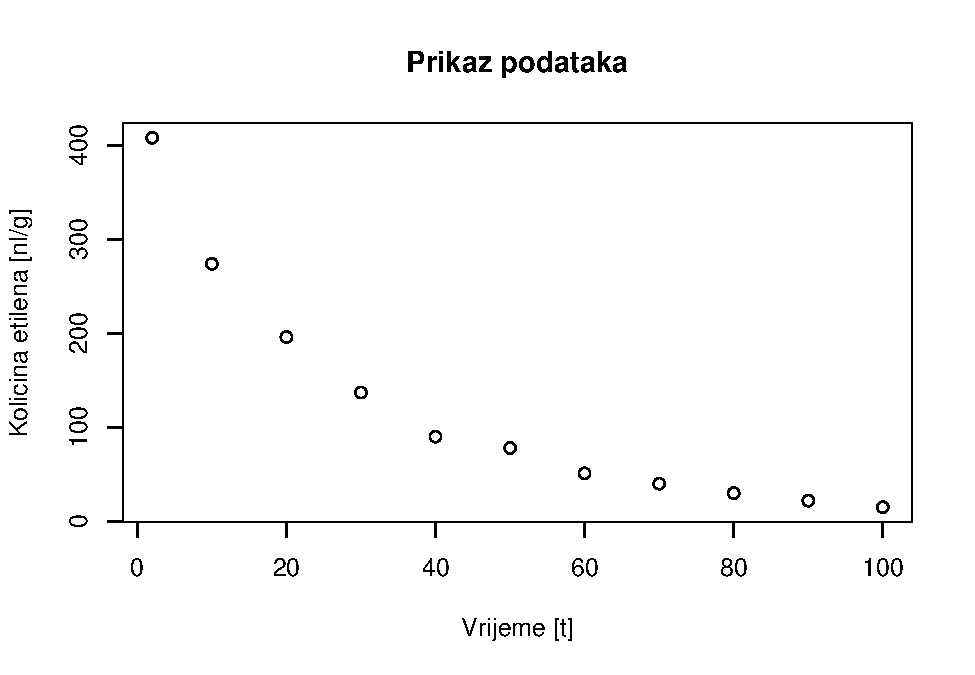
\includegraphics{Izvjestaj_files/figure-latex/unnamed-chunk-1-1.pdf}

\subsection{Prilagodba kvadratičnog
modela}\label{prilagodba-kvadraticnog-modela}

Prvi model čiju ćemo prilagodbu provesti jest slijedeći kvadratični
model: \[y = \theta_0 + \theta_1 x + \theta_2 x^2\]

\begin{Shaded}
\begin{Highlighting}[]
\NormalTok{X <-}\StringTok{ }\NormalTok{A.data$x}
\NormalTok{Y <-}\StringTok{ }\NormalTok{A.data$y}
\NormalTok{X.squared <-}\StringTok{ }\NormalTok{X^}\DecValTok{2}

\NormalTok{model <-}\StringTok{ }\KeywordTok{lm}\NormalTok{(Y ~}\StringTok{ }\NormalTok{X +}\StringTok{  }\NormalTok{X.squared)}
\end{Highlighting}
\end{Shaded}

Slijedeći graf prikazuje parabolu dobivenu prilagodbom navedenog modela
zajedno s empirijskim podacima:

\begin{Shaded}
\begin{Highlighting}[]
\NormalTok{predict.original <-}\StringTok{ }\NormalTok{function(x)\{}
  \NormalTok{beta0 <-}\StringTok{ }\NormalTok{model$coefficients[}\StringTok{"(Intercept)"}\NormalTok{]}
  \NormalTok{beta1 <-}\StringTok{ }\NormalTok{model$coefficients[}\StringTok{"X"}\NormalTok{]}
  \NormalTok{beta2 <-}\StringTok{ }\NormalTok{model$coefficients[}\StringTok{"X.squared"}\NormalTok{]}
  \KeywordTok{return}\NormalTok{(beta0 +}\StringTok{ }\NormalTok{beta1 *}\StringTok{ }\NormalTok{x +}\StringTok{ }\NormalTok{beta2 *}\StringTok{ }\NormalTok{x^}\DecValTok{2}\NormalTok{)}
\NormalTok{\}}

\KeywordTok{plot}\NormalTok{(X, Y, }\DataTypeTok{xlab =} \StringTok{"Vrijeme [t]"}\NormalTok{, }\DataTypeTok{ylab =} \StringTok{"Kolicina etilena [nl/g]"}\NormalTok{,}
     \DataTypeTok{main=}\StringTok{"Prilagodba modela"}\NormalTok{)}
\NormalTok{x.draw <-}\StringTok{ }\KeywordTok{min}\NormalTok{(X):}\KeywordTok{max}\NormalTok{(X)}
\NormalTok{y.draw <-}\StringTok{ }\KeywordTok{predict.original}\NormalTok{(x.draw)}
\KeywordTok{lines}\NormalTok{(x.draw, y.draw, }\DataTypeTok{col=}\StringTok{"red"}\NormalTok{)}
\end{Highlighting}
\end{Shaded}

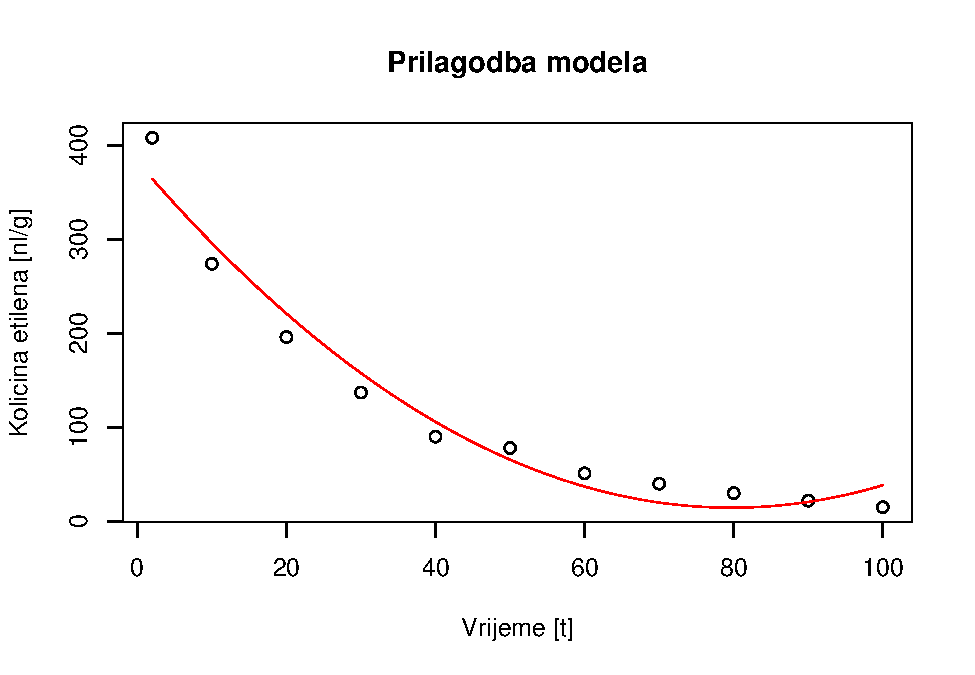
\includegraphics{Izvjestaj_files/figure-latex/unnamed-chunk-3-1.pdf}

\begin{Shaded}
\begin{Highlighting}[]
\KeywordTok{summary}\NormalTok{(model)}
\end{Highlighting}
\end{Shaded}

\begin{verbatim}
## 
## Call:
## lm(formula = Y ~ X + X.squared)
## 
## Residuals:
##     Min      1Q  Median      3Q     Max 
## -25.040 -21.335   1.353  14.753  43.637 
## 
## Coefficients:
##               Estimate Std. Error t value Pr(>|t|)    
## (Intercept) 382.605565  20.362603  18.790 6.65e-08 ***
## X            -9.237263   0.946518  -9.759 1.02e-05 ***
## X.squared     0.057950   0.009036   6.413 0.000206 ***
## ---
## Signif. codes:  0 '***' 0.001 '**' 0.01 '*' 0.05 '.' 0.1 ' ' 1
## 
## Residual standard error: 25.58 on 8 degrees of freedom
## Multiple R-squared:  0.9663, Adjusted R-squared:  0.9579 
## F-statistic: 114.7 on 2 and 8 DF,  p-value: 1.292e-06
\end{verbatim}

Testiramo slijedeću hipotezu: \(\theta_2 = 0\), uz dvostranu
alternativu. Kao što je vidljivo, p-vrijednost za parametar \(\theta_2\)
(koji stoji uz \(x^ 2\)) iznosi \(0.000206\). Prema tome, uz razinu
značajnosti ( \alpha = 5 \% ), odbacujemo nultu hipotezu u korist
alternative.

Također, iz priloženog sažetka doznajemo vrijednost statistike \(R^2\)
koja iznosi 0.9663. To je prilično zadovoljavajuća vrijednost iako
možemo bolje kao što ćemo vidjeti u nastavku.

\subsection{Provjera normalnosti
reziduala}\label{provjera-normalnosti-reziduala}

Pretpostavka linearne regresije jest da su reziduali normalno
distribuirani. Radi toga radimo provjeru normalnosti na sljedeća dva
načina: grafički (QQ plot) te Kolmogorov-Smirnovljevim testom.

\begin{Shaded}
\begin{Highlighting}[]
\KeywordTok{par}\NormalTok{(}\DataTypeTok{mfrow=}\KeywordTok{c}\NormalTok{(}\DecValTok{1}\NormalTok{,}\DecValTok{2}\NormalTok{))}
\KeywordTok{plot}\NormalTok{(X, model$residuals, }\DataTypeTok{xlab=}\StringTok{'Redni broj reziduala'}\NormalTok{, }\DataTypeTok{ylab =} \StringTok{'Iznos reziduala'}\NormalTok{,}
     \DataTypeTok{main =} \StringTok{'Graf reziduala'}\NormalTok{)}
\NormalTok{residuals.standardized <-}\StringTok{ }\KeywordTok{rstandard}\NormalTok{(model)}
\KeywordTok{plot}\NormalTok{(X, residuals.standardized, }\DataTypeTok{xlab=}\StringTok{'Redni broj reziduala'}\NormalTok{, }\DataTypeTok{ylab =} \StringTok{'Iznos reziduala'}\NormalTok{,}
     \DataTypeTok{main =} \StringTok{'Graf standardiziranih reziduala'}\NormalTok{)}
\end{Highlighting}
\end{Shaded}

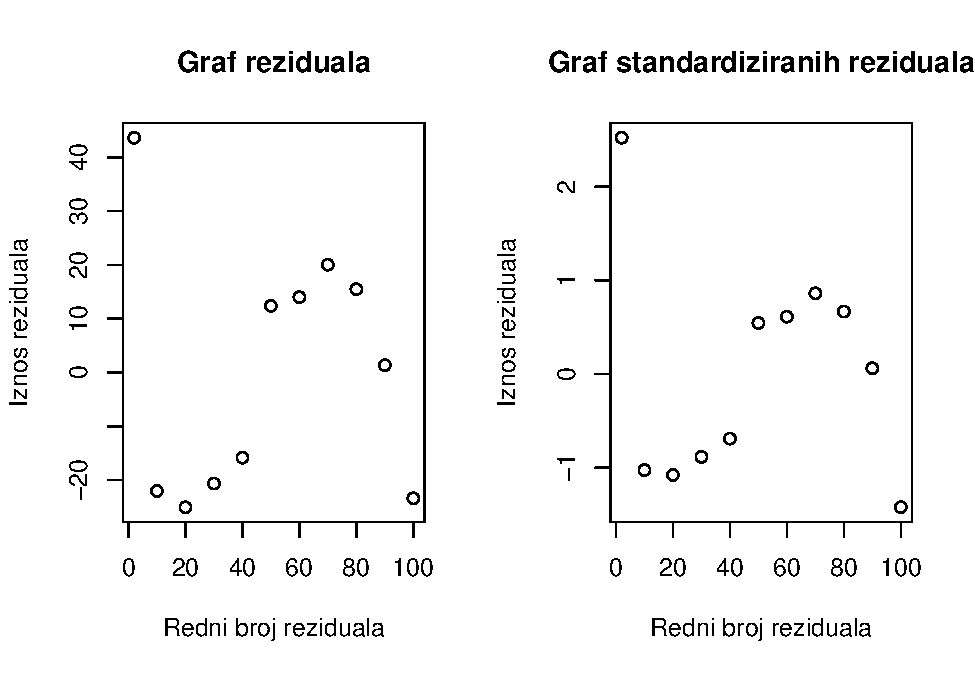
\includegraphics{Izvjestaj_files/figure-latex/unnamed-chunk-5-1.pdf}

\subsubsection{QQ plot}\label{qq-plot}

\begin{Shaded}
\begin{Highlighting}[]
\KeywordTok{qqnorm}\NormalTok{(residuals.standardized, }\DataTypeTok{xlab =} \StringTok{'Teoretski kvantili'}\NormalTok{, }\DataTypeTok{ylab =} \StringTok{'Kvantili iz uzorka'}\NormalTok{,}
       \DataTypeTok{main =} \StringTok{'QQ plot'}\NormalTok{)}
\KeywordTok{abline}\NormalTok{(}\DataTypeTok{a=}\DecValTok{0}\NormalTok{, }\DataTypeTok{b=}\DecValTok{1}\NormalTok{)}
\end{Highlighting}
\end{Shaded}

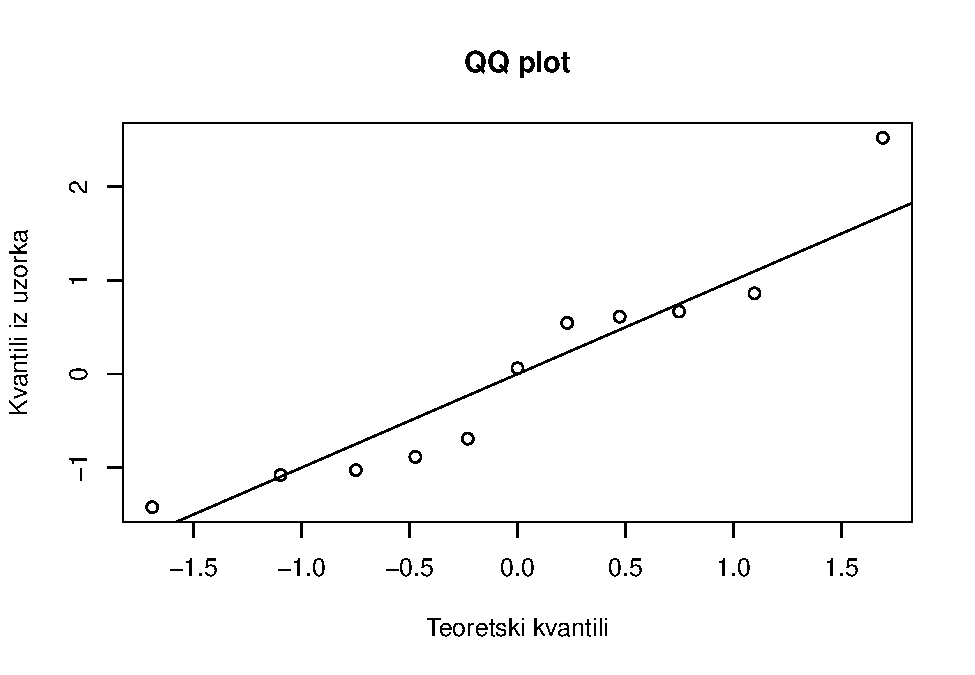
\includegraphics{Izvjestaj_files/figure-latex/unnamed-chunk-6-1.pdf}

Analizom dobivenog QQ plota, iako je uzorak relativno male veličine,
može se pretpostaviti da reziduali vrlo vjerojatno ne dolaze iz normalne
distribcije.

\subsubsection{Kolmogorov-Smirnovljev
test}\label{kolmogorov-smirnovljev-test}

\begin{Shaded}
\begin{Highlighting}[]
\KeywordTok{ks.test}\NormalTok{(residuals.standardized, }\StringTok{'pnorm'}\NormalTok{)}
\end{Highlighting}
\end{Shaded}

\begin{verbatim}
## 
##  One-sample Kolmogorov-Smirnov test
## 
## data:  residuals.standardized
## D = 0.20947, p-value = 0.6473
## alternative hypothesis: two-sided
\end{verbatim}

Provedbom Kolmogorov-Smirnovljevog testa dobivamo p-vrijednost jednaku
0.6473. Sa razinom značajnosti \(\alpha=5\%\) ne možemo odbaciti početnu
hipotezu da su reziduali normalno distribuirani u korist dvostrane
alternative.

\subsection{Logaritamska transformacija
podataka}\label{logaritamska-transformacija-podataka}

Slijedeće što ćemo napraviti jest transformirati originalni skup
podataka kako bi vidjeli ima li transformacija utjecaj na rezultate.
Transformacija koju ćemo koristi je slijedeća: \(y^0 = ln(y)\) .

\begin{Shaded}
\begin{Highlighting}[]
\NormalTok{Y0 <-}\StringTok{ }\KeywordTok{log}\NormalTok{(Y)}
\KeywordTok{plot}\NormalTok{(X, Y0, }\DataTypeTok{xlab =} \StringTok{"Vrijeme [t]"}\NormalTok{, }\DataTypeTok{ylab =} \StringTok{"Kolicina etilena [ln(nl/g)]"}\NormalTok{, }\DataTypeTok{main=}\StringTok{"Prikaz transformiranih podataka"}\NormalTok{)}
\end{Highlighting}
\end{Shaded}

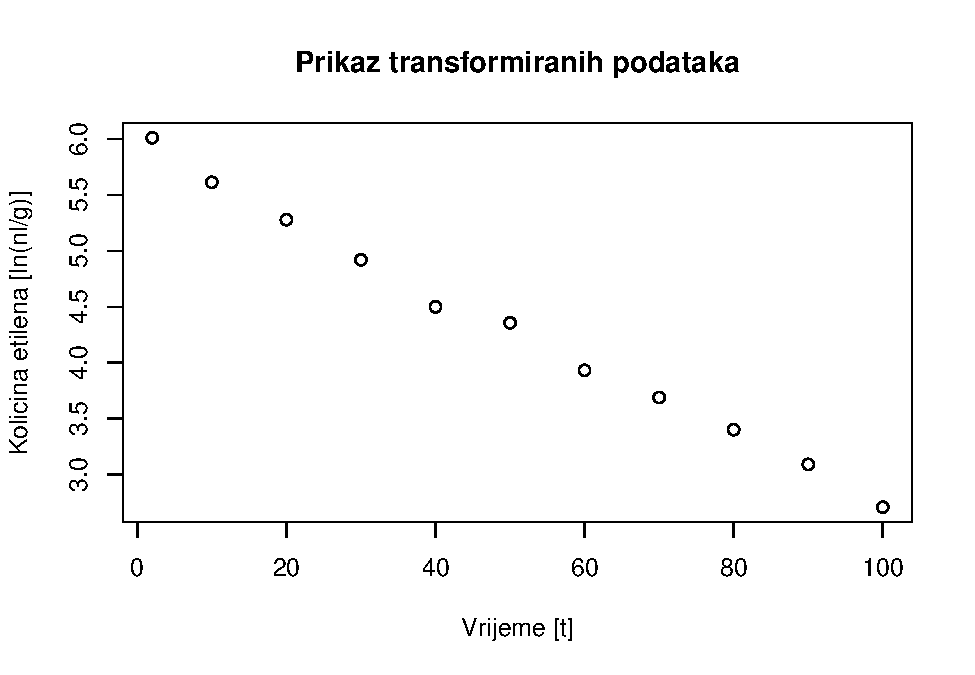
\includegraphics{Izvjestaj_files/figure-latex/unnamed-chunk-8-1.pdf}

Kao što je vidljivo na dijagramu raspršenja, nakon transformacije podaci
izgledaju puno bolje. Model kojeg ćemo u ovom slučaju iskoristiti glasi:
\[y^0 = \theta_0 + \theta_1 x\]

\begin{Shaded}
\begin{Highlighting}[]
\NormalTok{model.ln <-}\StringTok{ }\KeywordTok{lm}\NormalTok{(Y0 ~}\StringTok{ }\NormalTok{X)}

\NormalTok{predict.ln <-}\StringTok{ }\NormalTok{function(x)\{}
  \NormalTok{beta0 <-}\StringTok{ }\NormalTok{model.ln$coefficients[}\StringTok{"(Intercept)"}\NormalTok{]}
  \NormalTok{beta1 <-}\StringTok{ }\NormalTok{model.ln$coefficients[}\StringTok{"X"}\NormalTok{]}
  \KeywordTok{return}\NormalTok{(beta0 +}\StringTok{ }\NormalTok{beta1 *}\StringTok{ }\NormalTok{x)}
\NormalTok{\}}

\KeywordTok{plot}\NormalTok{(X, Y0, }\DataTypeTok{xlab =} \StringTok{"Vrijeme [t]"}\NormalTok{, }\DataTypeTok{ylab =} \StringTok{"Kolicina etilena [ln(nl/g)]"}\NormalTok{,}
     \DataTypeTok{main=}\StringTok{"Prilagodba modela"}\NormalTok{)}
\NormalTok{y.ln.draw <-}\StringTok{ }\KeywordTok{predict.ln}\NormalTok{(x.draw)}
\KeywordTok{lines}\NormalTok{(x.draw, y.ln.draw, }\DataTypeTok{col=}\StringTok{"red"}\NormalTok{)}
\end{Highlighting}
\end{Shaded}

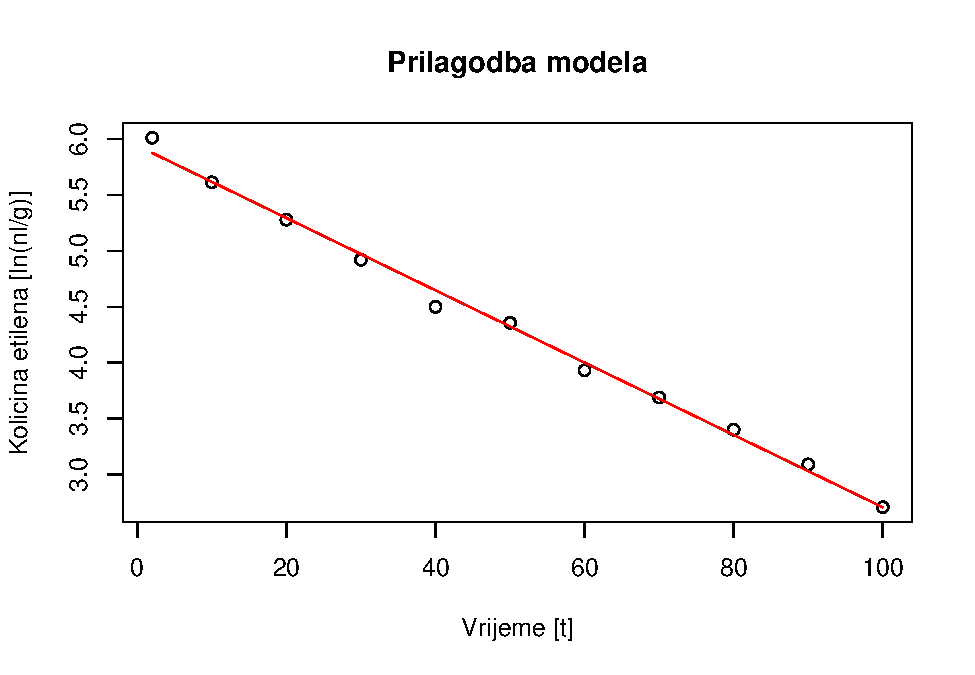
\includegraphics{Izvjestaj_files/figure-latex/unnamed-chunk-9-1.pdf}

\begin{Shaded}
\begin{Highlighting}[]
\KeywordTok{summary}\NormalTok{(model.ln)}
\end{Highlighting}
\end{Shaded}

\begin{verbatim}
## 
## Call:
## lm(formula = Y0 ~ X)
## 
## Residuals:
##       Min        1Q    Median        3Q       Max 
## -0.147537 -0.033230  0.000425  0.039823  0.135430 
## 
## Coefficients:
##               Estimate Std. Error t value Pr(>|t|)    
## (Intercept)  5.9404951  0.0443816   133.8 3.68e-16 ***
## X           -0.0323287  0.0007501   -43.1 9.73e-12 ***
## ---
## Signif. codes:  0 '***' 0.001 '**' 0.01 '*' 0.05 '.' 0.1 ' ' 1
## 
## Residual standard error: 0.07797 on 9 degrees of freedom
## Multiple R-squared:  0.9952, Adjusted R-squared:  0.9946 
## F-statistic:  1857 on 1 and 9 DF,  p-value: 9.734e-12
\end{verbatim}

Sada iz sažetka vidimo da je vrijednost \(R^2\) statistike jednaka
0.9952 što je puno bolje od prethodnog slučaja kada smo koristili
netrasnformirane podatake. Možemo biti zadovoljni pošto je ova
vrijednost vrlo blizu broju 1.

\subsection{Provjera normalnosti reziduala transformiranih
podataka}\label{provjera-normalnosti-reziduala-transformiranih-podataka}

Kao što smo napravili i za originalni skup podataka, provesti ćemo
provjeru normalnosti reziduala, ali sada za transformirane podatke.
Koristimo ista dva kriterija: grafički (QQ plot) te
Kolmogorov-Smirnovljev test.

\begin{Shaded}
\begin{Highlighting}[]
\KeywordTok{par}\NormalTok{(}\DataTypeTok{mfrow=}\KeywordTok{c}\NormalTok{(}\DecValTok{1}\NormalTok{,}\DecValTok{2}\NormalTok{))}
\KeywordTok{plot}\NormalTok{(X, model.ln$residuals, }\DataTypeTok{xlab=}\StringTok{'Redni broj reziduala'}\NormalTok{, }\DataTypeTok{ylab =} \StringTok{'Iznos reziduala'}\NormalTok{,}
     \DataTypeTok{main =} \StringTok{'Graf reziduala'}\NormalTok{)}
\NormalTok{residuals.ln.standardized <-}\StringTok{ }\KeywordTok{rstandard}\NormalTok{(model.ln)}
\KeywordTok{plot}\NormalTok{(X, residuals.ln.standardized, }\DataTypeTok{xlab=}\StringTok{'Redni broj reziduala'}\NormalTok{, }\DataTypeTok{ylab =} \StringTok{'Iznos reziduala'}\NormalTok{,}
     \DataTypeTok{main =} \StringTok{'Graf standardiziranih reziduala'}\NormalTok{)}
\end{Highlighting}
\end{Shaded}

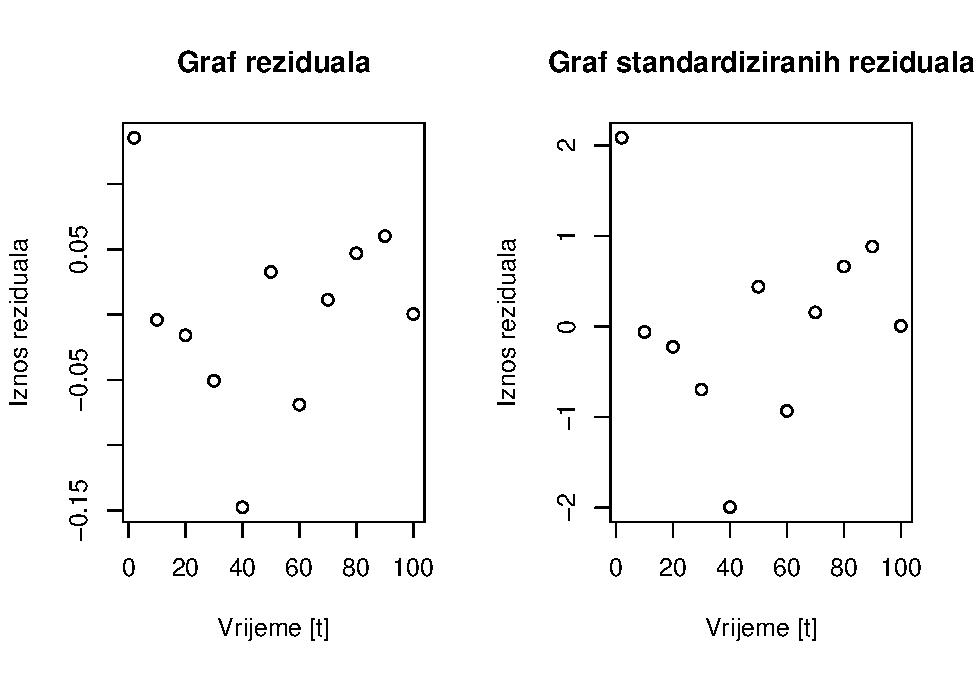
\includegraphics{Izvjestaj_files/figure-latex/unnamed-chunk-11-1.pdf}

Za razliku od reziduala originalnih podataka, reziduali logaritamski
transformiranih podataka pokazuju puno bolju distribuciju kao što je
vidljivo iz priloženih grafova.

\subsubsection{QQ plot}\label{qq-plot-1}

\begin{Shaded}
\begin{Highlighting}[]
\KeywordTok{qqnorm}\NormalTok{(residuals.ln.standardized, }\DataTypeTok{xlab =} \StringTok{'Teoretski kvantili'}\NormalTok{, }\DataTypeTok{ylab =} \StringTok{'Kvantili iz uzorka'}\NormalTok{,}
       \DataTypeTok{main =} \StringTok{'QQ plot'}\NormalTok{)}
\KeywordTok{abline}\NormalTok{(}\DataTypeTok{a=}\DecValTok{0}\NormalTok{, }\DataTypeTok{b=}\DecValTok{1}\NormalTok{)}
\end{Highlighting}
\end{Shaded}

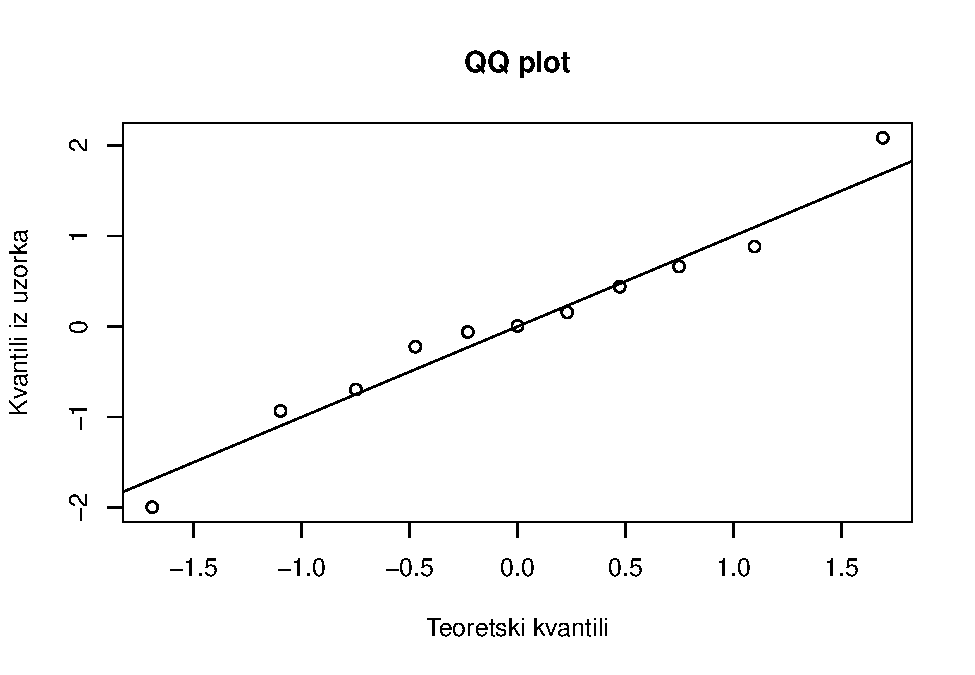
\includegraphics{Izvjestaj_files/figure-latex/unnamed-chunk-12-1.pdf}

Također, QQ plot reziduala transformiranih podataka pokazuje puno veće
podudaranje sa pravcem nego u slučaju netransformiranih podataka.

\subsubsection{Kolmogorov-Smirnovljev
test}\label{kolmogorov-smirnovljev-test-1}

\begin{Shaded}
\begin{Highlighting}[]
\KeywordTok{ks.test}\NormalTok{(residuals.ln.standardized, }\StringTok{'pnorm'}\NormalTok{)}
\end{Highlighting}
\end{Shaded}

\begin{verbatim}
## 
##  One-sample Kolmogorov-Smirnov test
## 
## data:  residuals.ln.standardized
## D = 0.13895, p-value = 0.9644
## alternative hypothesis: two-sided
\end{verbatim}

Provedbom Kolmogorov-Smirnovljevog testa nad transformiranim podacima,
dobivamo p-vrijednost u iznosu 0.9644. Slijedi da ne možemo na razini
značajnosti od ( \alpha = 5 \% ) odbaciti nultu hipotezu da su reziduali
normalno distribuirani u korist dvostrane alternative.

\subsection{Eksponencijalni model za originalne
podatke}\label{eksponencijalni-model-za-originalne-podatke}

Uz pretpostavku da je linearan model dobar za transformirane podatke,
njegova formula glasi:

\[\hat{y} = e^{5.9404951 - 0.0323287 \cdot x} \]

Na grafu ispod prikazani su parovi izmjerenih i procijenjenih podataka
\((y, \hat{y})\) uz pravac \(y=x\).

\begin{Shaded}
\begin{Highlighting}[]
\NormalTok{Y.predicted <-}\StringTok{ }\KeywordTok{predict.original}\NormalTok{(X)}
\KeywordTok{plot}\NormalTok{(Y, Y.predicted, }\DataTypeTok{xlab=}\StringTok{"y"}\NormalTok{, }\DataTypeTok{ylab=}\StringTok{"y_kapa"}\NormalTok{, }\DataTypeTok{main=}\StringTok{"Usporedba zadanih podataka i procjena"}\NormalTok{)}
\KeywordTok{abline}\NormalTok{(}\DataTypeTok{a=}\DecValTok{0}\NormalTok{, }\DataTypeTok{b=}\DecValTok{1}\NormalTok{)}
\end{Highlighting}
\end{Shaded}

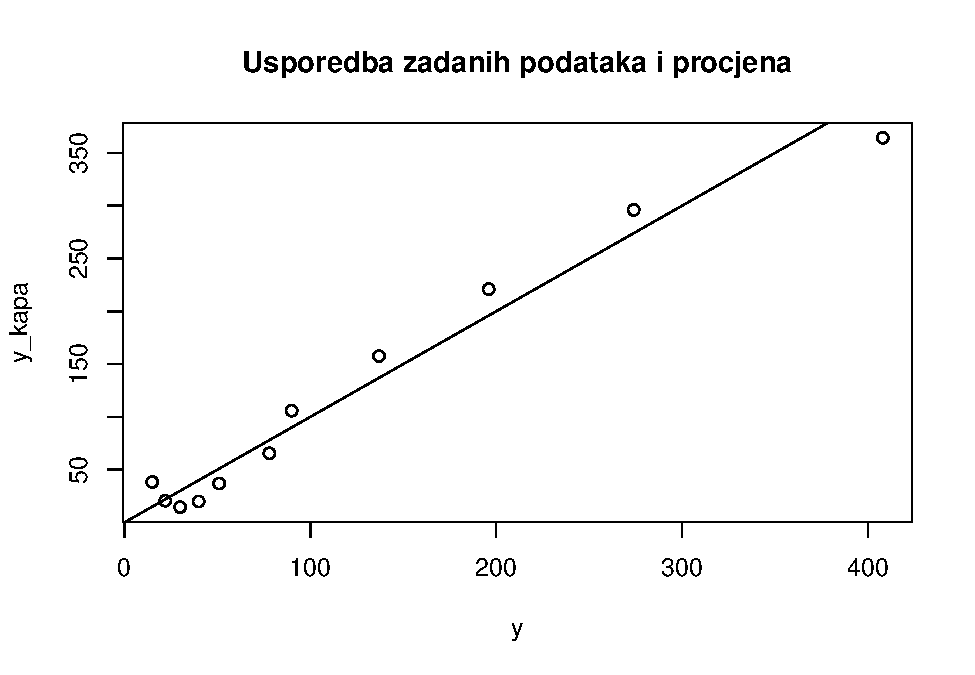
\includegraphics{Izvjestaj_files/figure-latex/unnamed-chunk-14-1.pdf}

\subsection{Krivulje 95\% pouzdanih
intervala}\label{krivulje-95-pouzdanih-intervala}

Na slijedećim grafovima prikazani su parovi podataka, i za originalne i
za transformirane podatke. Crnom bojom su označene gornja i donja
krivulja pouzdanosti za \(Y\) dok su zelenom bojom označene gornja i
donja krivulja pouzdanosti za \(\overline{Y}\).

\begin{Shaded}
\begin{Highlighting}[]
\NormalTok{X.new <-}\StringTok{ }\KeywordTok{seq}\NormalTok{(}\KeywordTok{min}\NormalTok{(X), }\KeywordTok{max}\NormalTok{(X))}
\NormalTok{X.squared.new <-}\StringTok{ }\NormalTok{X.new^}\DecValTok{2}

\NormalTok{prediction <-}\StringTok{ }\KeywordTok{predict.lm}\NormalTok{(model, }\DataTypeTok{newdata =} \KeywordTok{data.frame}\NormalTok{(}\DataTypeTok{X=}\NormalTok{X.new, }\DataTypeTok{X.squared=}\NormalTok{X.squared.new),}
                         \DataTypeTok{interval =} \StringTok{'prediction'}\NormalTok{, }\DataTypeTok{level=}\FloatTok{0.95}\NormalTok{)}
\NormalTok{confidence <-}\StringTok{ }\KeywordTok{predict.lm}\NormalTok{(model, }\DataTypeTok{newdata =} \KeywordTok{data.frame}\NormalTok{(}\DataTypeTok{X=}\NormalTok{X.new, }\DataTypeTok{X.squared=}\NormalTok{X.squared.new),}
                         \DataTypeTok{interval =} \StringTok{'confidence'}\NormalTok{, }\DataTypeTok{level=}\FloatTok{0.95}\NormalTok{)}
\KeywordTok{plot}\NormalTok{(X, Y, }\DataTypeTok{main=}\StringTok{'Model za originalne podatke'}\NormalTok{)}
\KeywordTok{lines}\NormalTok{(x.draw, y.draw, }\DataTypeTok{col=}\StringTok{"red"}\NormalTok{)}
\KeywordTok{lines}\NormalTok{(X.new, prediction[,}\DecValTok{2}\NormalTok{])}
\KeywordTok{lines}\NormalTok{(X.new, prediction[,}\DecValTok{3}\NormalTok{])}
\KeywordTok{lines}\NormalTok{(X.new, confidence[,}\DecValTok{2}\NormalTok{], }\DataTypeTok{col=}\StringTok{"green"}\NormalTok{)}
\KeywordTok{lines}\NormalTok{(X.new, confidence[,}\DecValTok{3}\NormalTok{], }\DataTypeTok{col=}\StringTok{"green"}\NormalTok{)}
\end{Highlighting}
\end{Shaded}

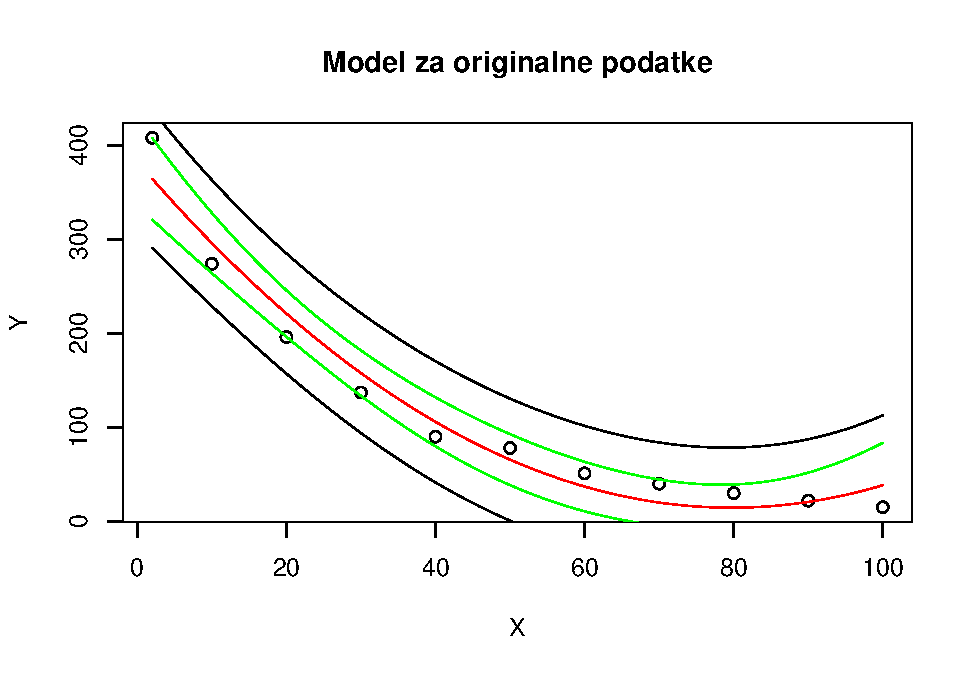
\includegraphics{Izvjestaj_files/figure-latex/unnamed-chunk-15-1.pdf}

\begin{Shaded}
\begin{Highlighting}[]
\NormalTok{prediction.ln <-}\StringTok{ }\KeywordTok{predict.lm}\NormalTok{(model.ln, }\DataTypeTok{newdata =} \KeywordTok{data.frame}\NormalTok{(}\DataTypeTok{X=}\NormalTok{X.new),}
                            \DataTypeTok{interval =} \StringTok{'prediction'}\NormalTok{, }\DataTypeTok{level=}\FloatTok{0.95}\NormalTok{)}
\NormalTok{confidence.ln <-}\StringTok{ }\KeywordTok{predict.lm}\NormalTok{(model.ln, }\DataTypeTok{newdata =} \KeywordTok{data.frame}\NormalTok{(}\DataTypeTok{X=}\NormalTok{X.new),}
                            \DataTypeTok{interval =} \StringTok{'confidence'}\NormalTok{, }\DataTypeTok{level=}\FloatTok{0.95}\NormalTok{)}
\KeywordTok{plot}\NormalTok{(X, Y0, }\DataTypeTok{main=}\StringTok{'Model za transformirane podatke'}\NormalTok{)}
\KeywordTok{lines}\NormalTok{(x.draw, y.ln.draw, }\DataTypeTok{col=}\StringTok{"red"}\NormalTok{)}
\KeywordTok{lines}\NormalTok{(X.new, prediction.ln[,}\DecValTok{2}\NormalTok{])}
\KeywordTok{lines}\NormalTok{(X.new, prediction.ln[,}\DecValTok{3}\NormalTok{])}
\KeywordTok{lines}\NormalTok{(X.new, confidence.ln[,}\DecValTok{2}\NormalTok{], }\DataTypeTok{col=}\StringTok{"green"}\NormalTok{)}
\KeywordTok{lines}\NormalTok{(X.new, confidence.ln[,}\DecValTok{3}\NormalTok{], }\DataTypeTok{col=}\StringTok{"green"}\NormalTok{)}
\end{Highlighting}
\end{Shaded}

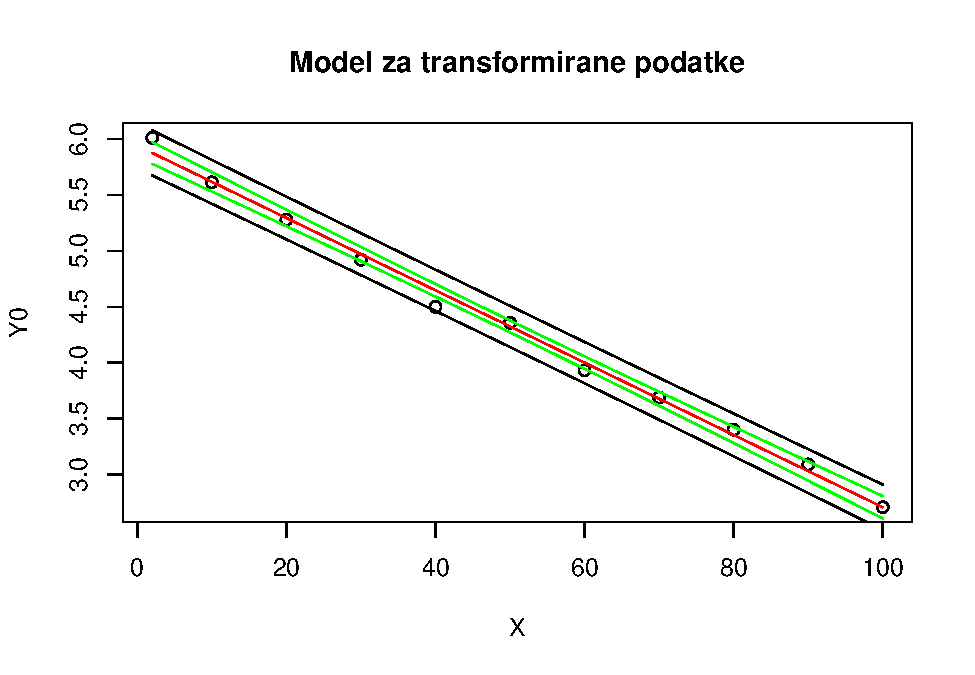
\includegraphics{Izvjestaj_files/figure-latex/unnamed-chunk-15-2.pdf}

Linearan model za transformirane podatke odnosno eksponencijalan model
za originalne podatke je zasigurno bolji. Osim što je iz grafova
vidljiva bolja prilagodba, 95\% pouzdani intervali za Y te srednju
vrijednost od Y su puno uži. Također, statistika \(R^2\) modela za
transformirane podatke iznosi 0.9952 dok za originalne podatke iznosi
0.9663.

\section{Zadatak B}\label{zadatak-b}

U članaku ``Determination of Biological Maturity and Effect of
Harvesting and Drying Conditions on Milling Quality of Paddy'' (J.
Agricultural Eng. Research, 1975., str. 353-361) obrađuju se podaci o
žetvi paddyja, vrste žita u Indiji. Varijabla x predstavlja datum žetve
(tj. to je broj dana proteklih od sjetve žita), a y predstavlja urod (u
kg/ha). Podaci se nalaze u datoteci zad55r.dat (Devore, Jay L.,
Probability and Statistics for Engineering and the Sciences, 1982.,
Brooks/Cole Publishing Company, Monterey, California, str. 478).

\subsection{Prikaz podataka u Kartezijevom koordinatnom
sustavu}\label{prikaz-podataka-u-kartezijevom-koordinatnom-sustavu-1}

Na slijedećem dijagramu prikazani su parovi podataka (x, y) iz zadanog
skupa:

\begin{Shaded}
\begin{Highlighting}[]
\NormalTok{B.data <-}\StringTok{ }\KeywordTok{read.table}\NormalTok{(}\StringTok{"zad55r.dat"}\NormalTok{, }\DataTypeTok{header =} \OtherTok{TRUE}\NormalTok{, }\DataTypeTok{sep =} \StringTok{" "}\NormalTok{)}
\NormalTok{B.data <-}\StringTok{ }\KeywordTok{data.frame}\NormalTok{(B.data)}

\KeywordTok{plot}\NormalTok{(B.data, }\DataTypeTok{xlab =} \StringTok{"broj dana proteklih od sjetve žita,(N)"}\NormalTok{, }\DataTypeTok{ylab =} \StringTok{"Urod,(kg/ha)"}\NormalTok{, }\DataTypeTok{main=}\StringTok{"Utjecaj datuma žetve na urod"}\NormalTok{)}
\end{Highlighting}
\end{Shaded}

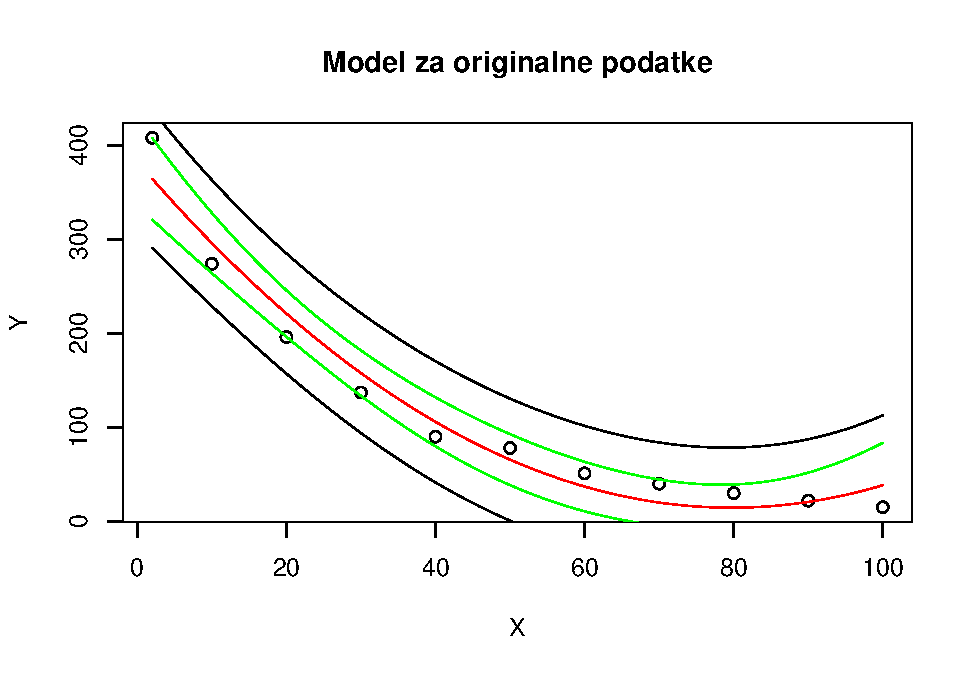
\includegraphics{Izvjestaj_files/figure-latex/unnamed-chunk-16-1.pdf}

\subsection{Prilagodba kvadratičnog
modela}\label{prilagodba-kvadraticnog-modela-1}

Prvi model čiju ćemo prilagodbu provesti jest sljedeći kvadratični
model: \[y = \theta_0 + \theta_1 x + \theta_2 x^2\]

\begin{Shaded}
\begin{Highlighting}[]
\NormalTok{urod <-}\StringTok{ }\NormalTok{B.data$y}
\NormalTok{N <-}\StringTok{ }\NormalTok{B.data$x}
\NormalTok{N.squared <-}\StringTok{ }\KeywordTok{I}\NormalTok{(N^}\DecValTok{2}\NormalTok{)}

\NormalTok{model <-}\StringTok{ }\KeywordTok{lm}\NormalTok{(urod ~}\StringTok{ }\NormalTok{N +}\StringTok{  }\NormalTok{N.squared)}
\end{Highlighting}
\end{Shaded}

Sljedeći graf prikazuje parabolu dobivenu prilagodbom navedenog modela s
empirijskim podacima:

\begin{Shaded}
\begin{Highlighting}[]
\NormalTok{f =}\StringTok{ }\NormalTok{function(x, koeficijenti)}
  \KeywordTok{return}\NormalTok{(koeficijenti[[}\DecValTok{1}\NormalTok{]] +}\StringTok{ }\NormalTok{koeficijenti[[}\DecValTok{2}\NormalTok{]] *}\StringTok{ }\NormalTok{x +}\StringTok{ }\NormalTok{koeficijenti[[}\DecValTok{3}\NormalTok{]] *}\StringTok{ }\NormalTok{x^}\DecValTok{2}\NormalTok{)}

\KeywordTok{plot}\NormalTok{(N, urod, }\DataTypeTok{xlab =} \StringTok{"broj dana proteklih od sjetve žita"}\NormalTok{, }\DataTypeTok{ylab =} \StringTok{"Urod, (kg/ha)"}\NormalTok{,}
     \DataTypeTok{main=}\StringTok{"Utjecaj datuma žetve na urod"}\NormalTok{)}
\KeywordTok{curve}\NormalTok{(}\KeywordTok{f}\NormalTok{(x, model$coefficients), }\DataTypeTok{add =} \OtherTok{TRUE}\NormalTok{, }\DataTypeTok{col =} \StringTok{"red"}\NormalTok{)}
\end{Highlighting}
\end{Shaded}

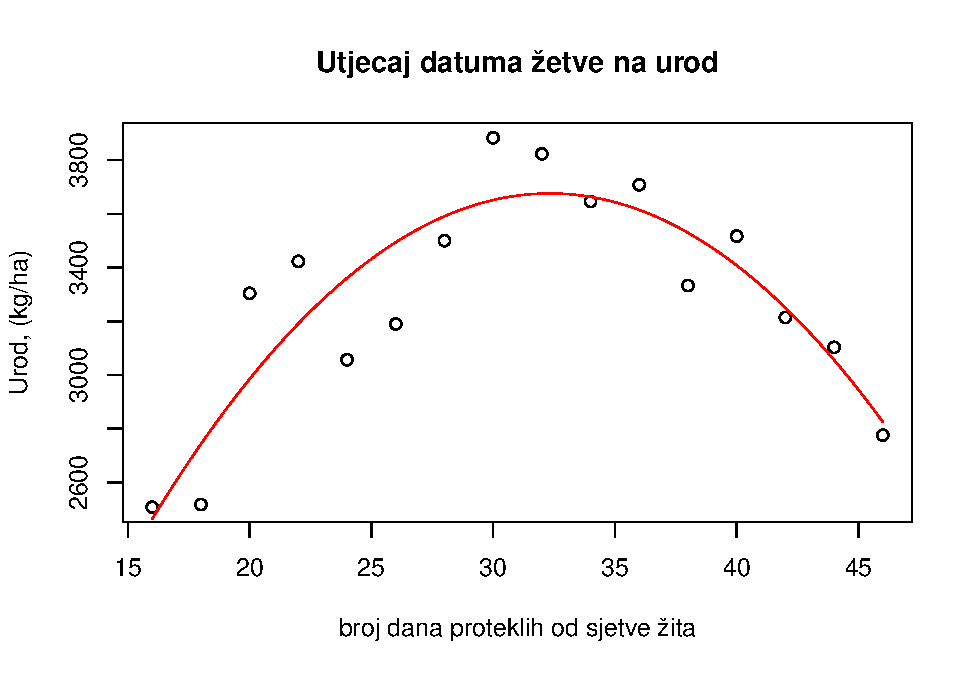
\includegraphics{Izvjestaj_files/figure-latex/unnamed-chunk-18-1.pdf}

\subsection{Provjera normalnosti
reziduala}\label{provjera-normalnosti-reziduala-1}

Pretpostavka linearne regresije jest da su reziduali normalno
distribuirani. Radi toga radimo provjeru normalnosti na sljedeća dva
načina: grafički (QQ plot) te Kolmogorov-Smirnovljevim testom.

\begin{Shaded}
\begin{Highlighting}[]
\KeywordTok{par}\NormalTok{(}\DataTypeTok{mfrow=}\KeywordTok{c}\NormalTok{(}\DecValTok{1}\NormalTok{,}\DecValTok{2}\NormalTok{))}

\KeywordTok{plot}\NormalTok{(N, model$residuals, }\DataTypeTok{xlab=}\StringTok{'Redni broj reziduala'}\NormalTok{, }\DataTypeTok{ylab =} \StringTok{'Iznos reziduala'}\NormalTok{,}
     \DataTypeTok{main =} \StringTok{'Graf reziduala'}\NormalTok{)}

\KeywordTok{plot}\NormalTok{(N, }\KeywordTok{rstandard}\NormalTok{(model), }\DataTypeTok{xlab=}\StringTok{'Redni broj reziduala'}\NormalTok{, }\DataTypeTok{ylab =} \StringTok{'Iznos reziduala'}\NormalTok{,}
     \DataTypeTok{main =} \StringTok{'Graf standardiziranih reziduala'}\NormalTok{)}
\end{Highlighting}
\end{Shaded}

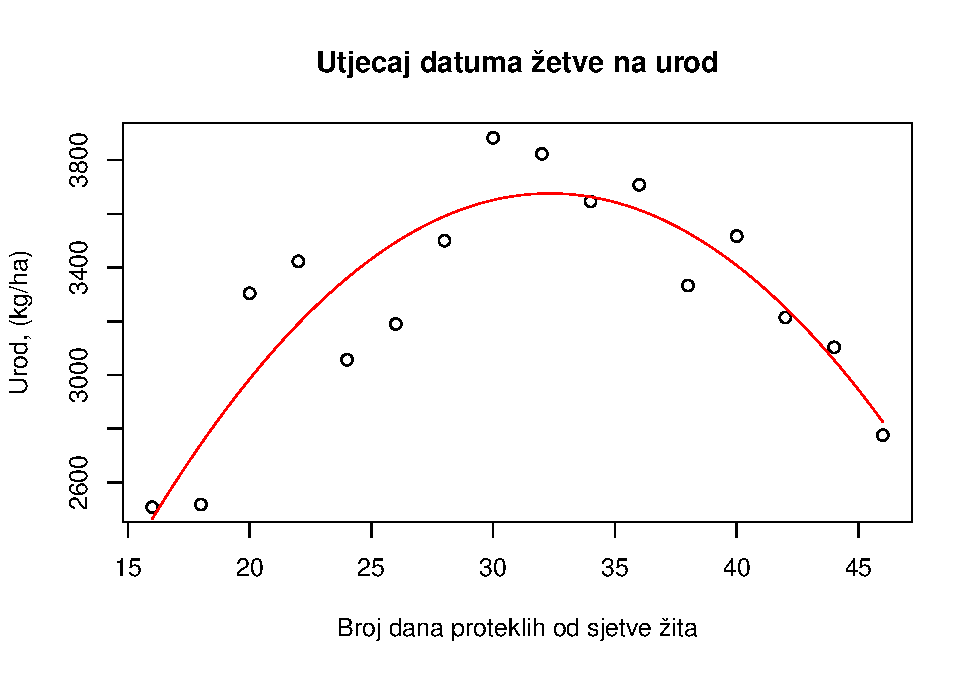
\includegraphics{Izvjestaj_files/figure-latex/unnamed-chunk-19-1.pdf}

\subsubsection{QQ plot}\label{qq-plot-2}

\begin{Shaded}
\begin{Highlighting}[]
\KeywordTok{qqnorm}\NormalTok{(}\KeywordTok{rstandard}\NormalTok{(model), }\DataTypeTok{xlab =} \StringTok{'Teoretski kvantili'}\NormalTok{, }\DataTypeTok{ylab =} \StringTok{'Kvantili iz uzorka'}\NormalTok{,}
       \DataTypeTok{main =} \StringTok{'QQ plot'}\NormalTok{)}
\KeywordTok{abline}\NormalTok{(}\DataTypeTok{a=}\DecValTok{0}\NormalTok{, }\DataTypeTok{b=}\DecValTok{1}\NormalTok{)}
\end{Highlighting}
\end{Shaded}

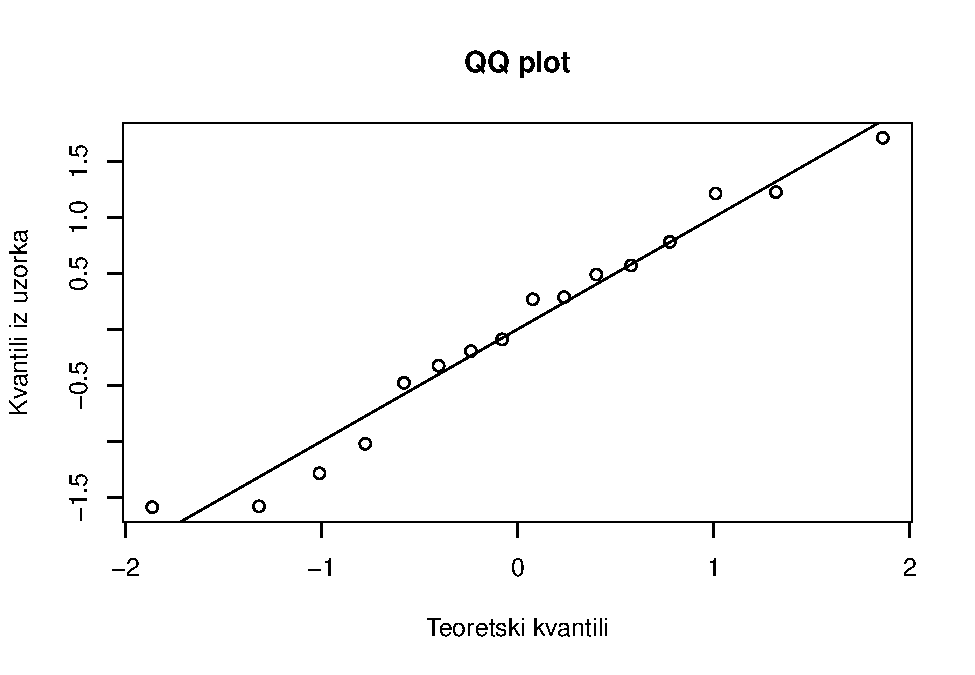
\includegraphics{Izvjestaj_files/figure-latex/unnamed-chunk-20-1.pdf}
Analizom dobivenog QQ plota može se pretpostaviti da reziduali dolaze iz
normalne distribcije.

\subsubsection{Kolmogorov-Smirnovljev
test}\label{kolmogorov-smirnovljev-test-2}

\begin{Shaded}
\begin{Highlighting}[]
\KeywordTok{ks.test}\NormalTok{(}\KeywordTok{rstandard}\NormalTok{(model), }\StringTok{'pnorm'}\NormalTok{)}
\end{Highlighting}
\end{Shaded}

\begin{verbatim}
## 
##  One-sample Kolmogorov-Smirnov test
## 
## data:  rstandard(model)
## D = 0.10553, p-value = 0.9857
## alternative hypothesis: two-sided
\end{verbatim}

Provedbom Kolmogorov-Smirnovljevog testa dobivamo p-vrijednost jednaku
0.9857. Test na normalnost za reziduale ne može odbaciti H0 da
standardizirani reziduali dolaze iz normalne razdiobe.

\subsection{\texorpdfstring{Hipoteza
\(H_0 : \theta_2 = 0\)}{Hipoteza H\_0 : \textbackslash{}theta\_2 = 0}}\label{hipoteza-h_0-theta_2-0}

\begin{Shaded}
\begin{Highlighting}[]
\KeywordTok{summary}\NormalTok{(model)}
\end{Highlighting}
\end{Shaded}

\begin{verbatim}
## 
## Call:
## lm(formula = urod ~ N + N.squared)
## 
## Residuals:
##     Min      1Q  Median      3Q     Max 
## -304.00 -117.23   13.32  118.63  318.73 
## 
## Coefficients:
##               Estimate Std. Error t value Pr(>|t|)    
## (Intercept) -1074.6320   618.0231  -1.739    0.106    
## N             293.9240    42.2303   6.960 9.92e-06 ***
## N.squared      -4.5464     0.6753  -6.733 1.40e-05 ***
## ---
## Signif. codes:  0 '***' 0.001 '**' 0.01 '*' 0.05 '.' 0.1 ' ' 1
## 
## Residual standard error: 204.1 on 13 degrees of freedom
## Multiple R-squared:  0.7939, Adjusted R-squared:  0.7622 
## F-statistic: 25.03 on 2 and 13 DF,  p-value: 3.483e-05
\end{verbatim}

Testiramo sljedeću hipotezu: \(H_0 : \theta_2 = 0\), u odnosu na
alternativu \(H_a : \theta_2 != 0\). Kao što je vidljivo, p-vrijednost
za parametar \(\theta_2\) (koji stoji uz ( x\^{}2 )) iznosi
\(1.40\cdot10^{-5}\). Prema tome, uz razinu značajnosti ( \alpha = 1 \%
), odbacujemo nultu hipotezu u korist alternative. \(theta_2\) je
značajan koeficijent.

\subsection{Krivulje 95\% pouzdanih
intervala}\label{krivulje-95-pouzdanih-intervala-1}

\begin{Shaded}
\begin{Highlighting}[]
\KeywordTok{plot}\NormalTok{(N,urod)}
\NormalTok{prediction =}\StringTok{ }\KeywordTok{predict.lm}\NormalTok{(model,B.data,}\DataTypeTok{interval =} \StringTok{"prediction"}\NormalTok{)}
\NormalTok{confidence =}\StringTok{ }\KeywordTok{predict.lm}\NormalTok{(model,B.data,}\DataTypeTok{interval =} \StringTok{"confidence"}\NormalTok{)}

\KeywordTok{curve}\NormalTok{(}\KeywordTok{f}\NormalTok{(x, model$coefficients), }\DataTypeTok{add =} \OtherTok{TRUE}\NormalTok{, }\DataTypeTok{col =} \StringTok{"red"}\NormalTok{)}
\KeywordTok{lines}\NormalTok{(N, prediction[,}\DecValTok{2}\NormalTok{])}
\KeywordTok{lines}\NormalTok{(N, prediction[,}\DecValTok{3}\NormalTok{])}
\KeywordTok{lines}\NormalTok{(N, confidence[,}\DecValTok{2}\NormalTok{], }\DataTypeTok{col=}\StringTok{"green"}\NormalTok{)}
\KeywordTok{lines}\NormalTok{(N, confidence[,}\DecValTok{3}\NormalTok{], }\DataTypeTok{col=}\StringTok{"green"}\NormalTok{)}
\end{Highlighting}
\end{Shaded}

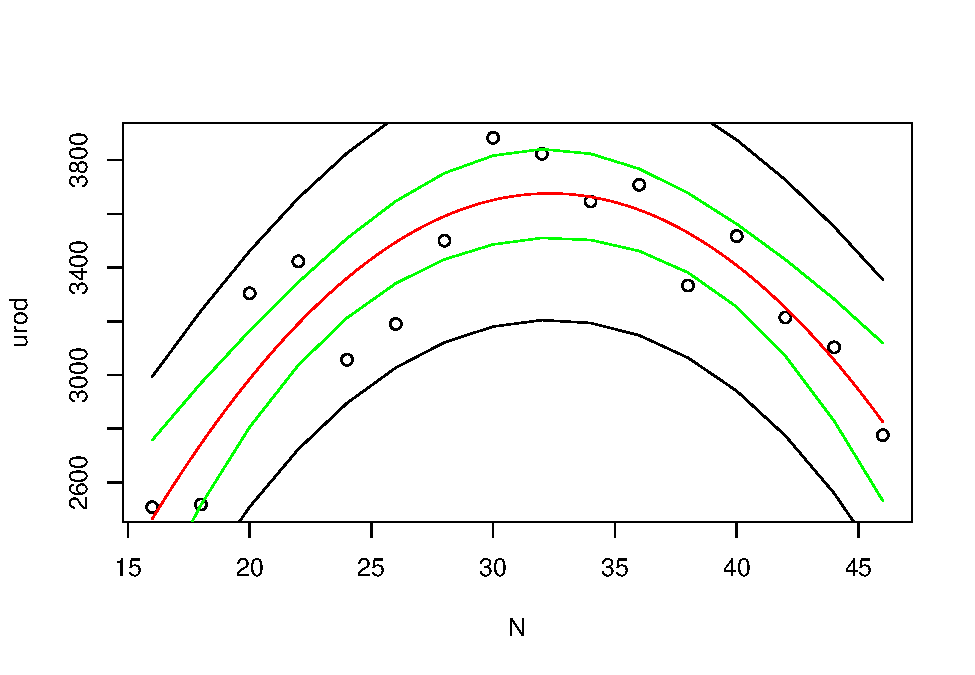
\includegraphics{Izvjestaj_files/figure-latex/unnamed-chunk-23-1.pdf}

\subsection{Zaključak}\label{zakljucak}

Iz prethodne analize podataka možemo zaključiti da postoji kvadratna
veza između uroda i broj dana proteklih od sjetve žita te time
opravdavamo optimalno razdoblje žetve između 28 i 36 nakon cvatnje.

\section{Zadatak C}\label{zadatak-c}

U radu ``An Ultracentrifuge Flour Absorption Method'' (Cereal Chemistry,
1978., str. 96-101) autori su proučavali odnos između apsorpcije vode
pšeničnog brašna i raznih karakteristika tog brašna. Konkretno,
promatrali su odnos između apsorpcije z (u \%) te proteina brašna x (u
\%) i gubitka škroba y (u Farrandovim jedinicama). Podaci dobiveni
pokusom nalaze se u datoteci zad57r.dat (Devore, Jay L., Probability and
Statistics for Engineering and the Sciences, 1982., Brooks/Cole
Publishing Company, Monterey, California, str. 490).

\subsection{Prikaz podataka u Kartezijevom koordinatnom sustavu (2D i
3D)}\label{prikaz-podataka-u-kartezijevom-koordinatnom-sustavu-2d-i-3d}

Na početku zadatka ćemo dane podatke prikazati u 2D koordinatnom sustavu
(X,Y), (X,Z) i (Y,Z) te zatim sve podatke zajedno u 3D koordinatnom
sustavu (X,Y,Z).

\begin{Shaded}
\begin{Highlighting}[]
\NormalTok{C.data <-}\StringTok{ }\KeywordTok{read.table}\NormalTok{(}\StringTok{"zad57r.dat"}\NormalTok{, }\DataTypeTok{header =} \OtherTok{TRUE}\NormalTok{, }\DataTypeTok{sep =} \StringTok{" "}\NormalTok{)}
\NormalTok{C.data <-}\StringTok{ }\KeywordTok{data.frame}\NormalTok{(C.data)}

\NormalTok{X <-}\StringTok{ }\NormalTok{C.data$x}
\NormalTok{Y <-}\StringTok{ }\NormalTok{C.data$y}
\NormalTok{Z <-}\StringTok{ }\NormalTok{C.data$z}

\KeywordTok{plot} \NormalTok{(X,Z, }\DataTypeTok{xlab =} \StringTok{"proteini brašna [%]"}\NormalTok{,}\DataTypeTok{ylab =} \StringTok{"apsorpcija [%]"}\NormalTok{, }\DataTypeTok{main=}\StringTok{"Prikaz podataka X,Z"}\NormalTok{)}
\end{Highlighting}
\end{Shaded}

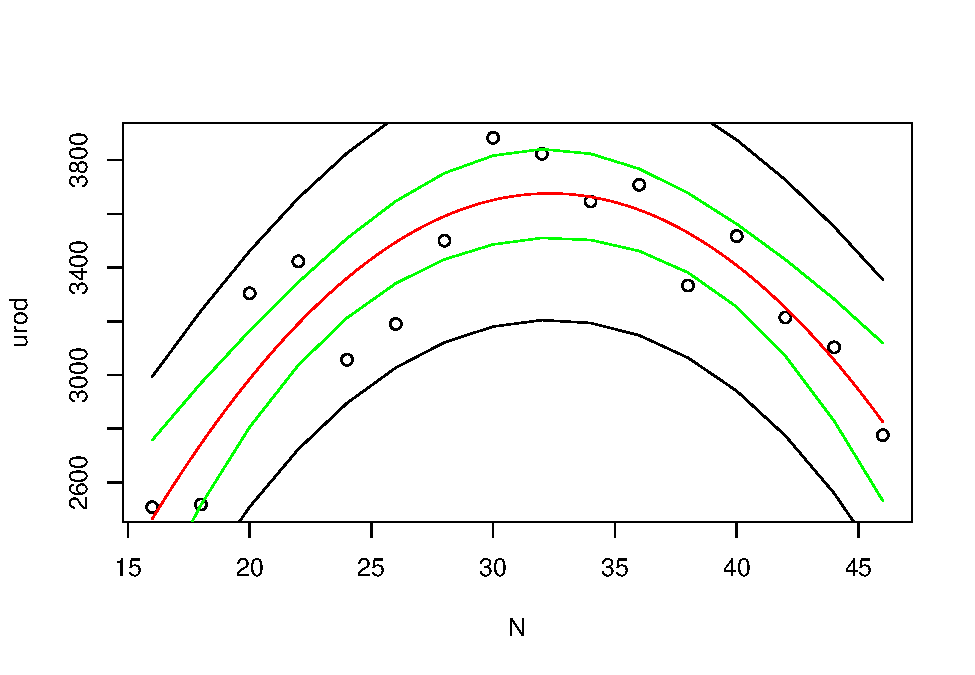
\includegraphics{Izvjestaj_files/figure-latex/unnamed-chunk-24-1.pdf}

\begin{Shaded}
\begin{Highlighting}[]
\KeywordTok{plot} \NormalTok{(Y,Z, }\DataTypeTok{xlab =} \StringTok{"gubitak škroba [Farrandove jedinice]"}\NormalTok{,}\DataTypeTok{ylab =} \StringTok{"apsorpcija [%]"}\NormalTok{, }\DataTypeTok{main=}\StringTok{"Prikaz podataka Y,Z"}\NormalTok{)}
\end{Highlighting}
\end{Shaded}

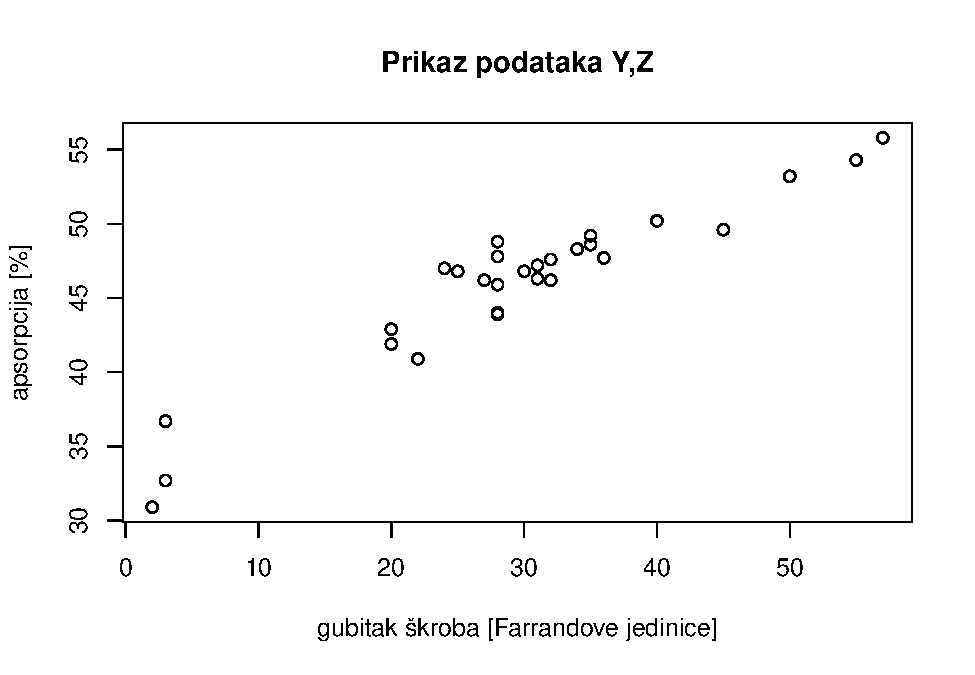
\includegraphics{Izvjestaj_files/figure-latex/unnamed-chunk-24-2.pdf}

\begin{Shaded}
\begin{Highlighting}[]
\KeywordTok{plot} \NormalTok{(X,Y, }\DataTypeTok{xlab =} \StringTok{"proteini brašna [%]"}\NormalTok{,}\DataTypeTok{ylab =} \StringTok{"gubitak škroba [Farrandove jedinice]"}\NormalTok{, }\DataTypeTok{main=}\StringTok{"Prikaz podataka X,Y"}\NormalTok{)}
\end{Highlighting}
\end{Shaded}

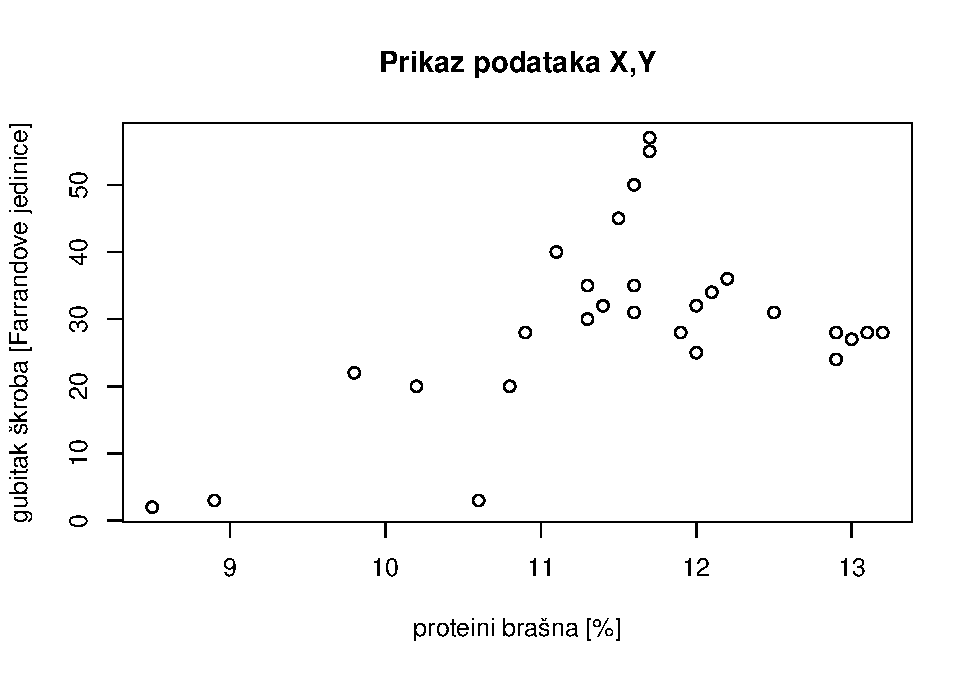
\includegraphics{Izvjestaj_files/figure-latex/unnamed-chunk-24-3.pdf}

\begin{Shaded}
\begin{Highlighting}[]
\KeywordTok{require}\NormalTok{(scatterplot3d)}
\end{Highlighting}
\end{Shaded}

\begin{verbatim}
## Loading required package: scatterplot3d
\end{verbatim}

\begin{verbatim}
## Warning: package 'scatterplot3d' was built under R version 3.3.3
\end{verbatim}

\begin{Shaded}
\begin{Highlighting}[]
\KeywordTok{scatterplot3d}\NormalTok{(X,Y,Z, }\DataTypeTok{pch =} \DecValTok{19}\NormalTok{, }\DataTypeTok{color =} \StringTok{"green4"}\NormalTok{, }\DataTypeTok{xlab=}\StringTok{"proteini brašna [%]"}\NormalTok{,}\DataTypeTok{ylab=}\StringTok{"gubitak škroba [Farrandove jedinice]"}\NormalTok{,}\DataTypeTok{zlab =} \StringTok{"apsorpcija [%]"}\NormalTok{,}\DataTypeTok{main =}\StringTok{"Prikaz podataka X,Y,Z"} \NormalTok{)}
\end{Highlighting}
\end{Shaded}

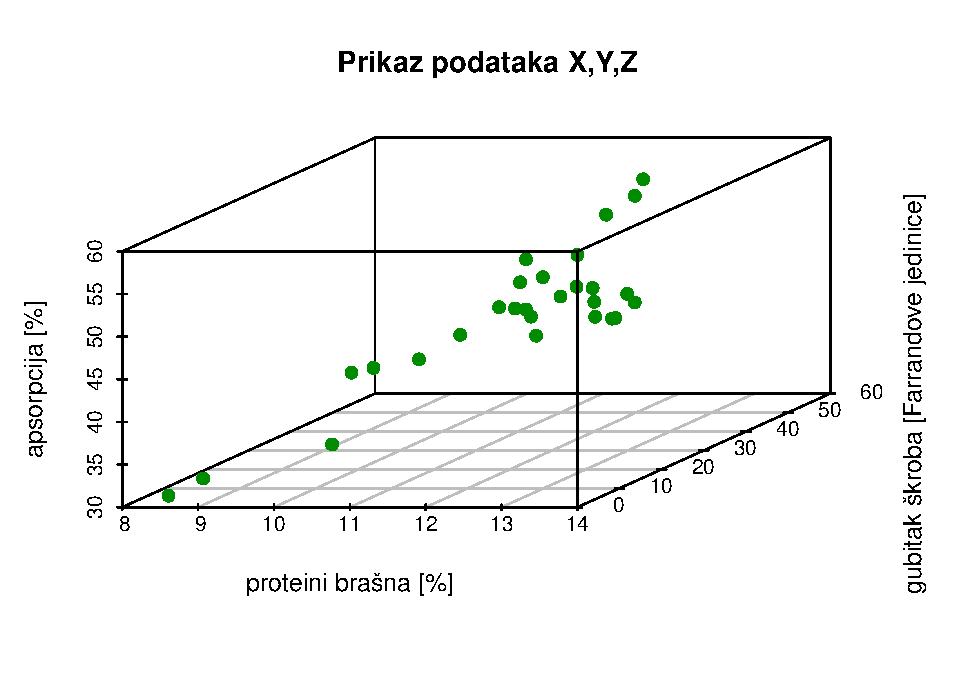
\includegraphics{Izvjestaj_files/figure-latex/unnamed-chunk-24-4.pdf}
\#\# Testovi korelacije

Zatim ćemo nad parom (Y,Z) provesti Pearsonov test korelacije, a nad
parom (X,Y) Spearmanov test korelacije.

\begin{Shaded}
\begin{Highlighting}[]
\KeywordTok{cor}\NormalTok{(Y,Z)}
\end{Highlighting}
\end{Shaded}

\begin{verbatim}
## [1] 0.946518
\end{verbatim}

\begin{Shaded}
\begin{Highlighting}[]
\KeywordTok{cor.test}\NormalTok{(Y,Z)}
\end{Highlighting}
\end{Shaded}

\begin{verbatim}
## 
##  Pearson's product-moment correlation
## 
## data:  Y and Z
## t = 14.958, df = 26, p-value = 2.751e-14
## alternative hypothesis: true correlation is not equal to 0
## 95 percent confidence interval:
##  0.8864776 0.9752210
## sample estimates:
##      cor 
## 0.946518
\end{verbatim}

Nad parom (Y,Z) smo radili Pearsonov test korelacije. Iz dobivenih
rezultata vidimo da je \(r\) = 0.946518 te zaključujemo da su podaci
pozitivno korelirani. P-vrijednost iz testa koreliranosti je jako mala
(\(2.751e-14\)) pa možemo odbaciti hipotezu da je koreliranost jednaka
0. Možemo primjetiti povezanost između velike korelacije i male
p-vrijednosti.

\begin{Shaded}
\begin{Highlighting}[]
\KeywordTok{cor}\NormalTok{(X,Y,}\DataTypeTok{method =} \StringTok{"spearman"}\NormalTok{)}
\end{Highlighting}
\end{Shaded}

\begin{verbatim}
## [1] 0.2870111
\end{verbatim}

\begin{Shaded}
\begin{Highlighting}[]
\KeywordTok{cor.test}\NormalTok{(X,Y,}\DataTypeTok{method =} \StringTok{"spearman"}\NormalTok{)}
\end{Highlighting}
\end{Shaded}

\begin{verbatim}
## Warning in cor.test.default(X, Y, method = "spearman"): Cannot compute
## exact p-value with ties
\end{verbatim}

\begin{verbatim}
## 
##  Spearman's rank correlation rho
## 
## data:  X and Y
## S = 2605.3, p-value = 0.1386
## alternative hypothesis: true rho is not equal to 0
## sample estimates:
##       rho 
## 0.2870111
\end{verbatim}

\begin{Shaded}
\begin{Highlighting}[]
\NormalTok{sumY =}\StringTok{ }\KeywordTok{rnorm}\NormalTok{(}\DecValTok{28}\NormalTok{,}\DecValTok{0}\NormalTok{,}\FloatTok{0.01}\NormalTok{);}
\NormalTok{sumX =}\StringTok{ }\KeywordTok{rnorm}\NormalTok{(}\DecValTok{28}\NormalTok{,}\DecValTok{0}\NormalTok{,}\FloatTok{0.01}\NormalTok{);}

\NormalTok{noviX=X+sumX}
\NormalTok{noviY=Y+sumY}

\KeywordTok{cor}\NormalTok{(noviX,noviY,}\DataTypeTok{method =} \StringTok{"spearman"}\NormalTok{)}
\end{Highlighting}
\end{Shaded}

\begin{verbatim}
## [1] 0.30104
\end{verbatim}

\begin{Shaded}
\begin{Highlighting}[]
\KeywordTok{cor.test}\NormalTok{(noviX,noviY,}\DataTypeTok{method =} \StringTok{"spearman"}\NormalTok{)}
\end{Highlighting}
\end{Shaded}

\begin{verbatim}
## 
##  Spearman's rank correlation rho
## 
## data:  noviX and noviY
## S = 2554, p-value = 0.1196
## alternative hypothesis: true rho is not equal to 0
## sample estimates:
##     rho 
## 0.30104
\end{verbatim}

Nad parom (X,Y) smo radili Spearmanov test korelacije. Pomoću rezultata
naslućujemo da je korelacija između danih podataka jako mala jer je
\(r\) = 0.2870111. P-vrijednost testa je 0.1386 pa ne možemo odbaciti
hipotezu da je korelacija jednaka 0. Problem kod Spearmanovog testa je
što ne može naći egzaktnu p-vrijednost ako ima jednake vrijendosti. Zbog
toga smo napravili šum za obje varijable X i Y koji je iz normalne
distribucije \(N (0, 0.0001)\). Ponovno smo izračunali stupanj
korelacije i napravili Spearmanov test. Novo dobivene vrijednosti se
malo razlikuju od prijašnjih pa zbog p-vrijednosti veće od 0.05 ne
možemo zaključiti da je korelacija različita od 0.

\subsection{Prilagodba linearnog
modela}\label{prilagodba-linearnog-modela}

Sljedeći korak našeg zadatka su prilagodbe linearnih modela. Prvi model
čiju ćemo prilagodbu provesti jest slijedeći linearni model:
\[z = \alpha_0 + \alpha_1 x \]

\begin{Shaded}
\begin{Highlighting}[]
\NormalTok{X <-}\StringTok{ }\NormalTok{C.data$x}
\NormalTok{Z <-}\StringTok{ }\NormalTok{C.data$z}

\NormalTok{model <-}\StringTok{ }\KeywordTok{lm} \NormalTok{(Z ~}\StringTok{ }\NormalTok{X)}
\end{Highlighting}
\end{Shaded}

Sljedeći graf prikazuje pravac dobiven prilagodbom navedenog modela
zajedno s empirijskim podacima. Dobili smo pravac
\(z = 3.321*x + 7.753\).

\begin{Shaded}
\begin{Highlighting}[]
\KeywordTok{plot}\NormalTok{(X, Z, }\DataTypeTok{xlab =} \StringTok{"proteini brašna [%]"}\NormalTok{, }\DataTypeTok{ylab =} \StringTok{"Apsorpcija [%]"}\NormalTok{,}
     \DataTypeTok{main=}\StringTok{"Prilagodba modela"}\NormalTok{)}
\KeywordTok{lines}\NormalTok{(X, model$fitted.values, }\DataTypeTok{col=}\StringTok{"red"}\NormalTok{)}
\end{Highlighting}
\end{Shaded}

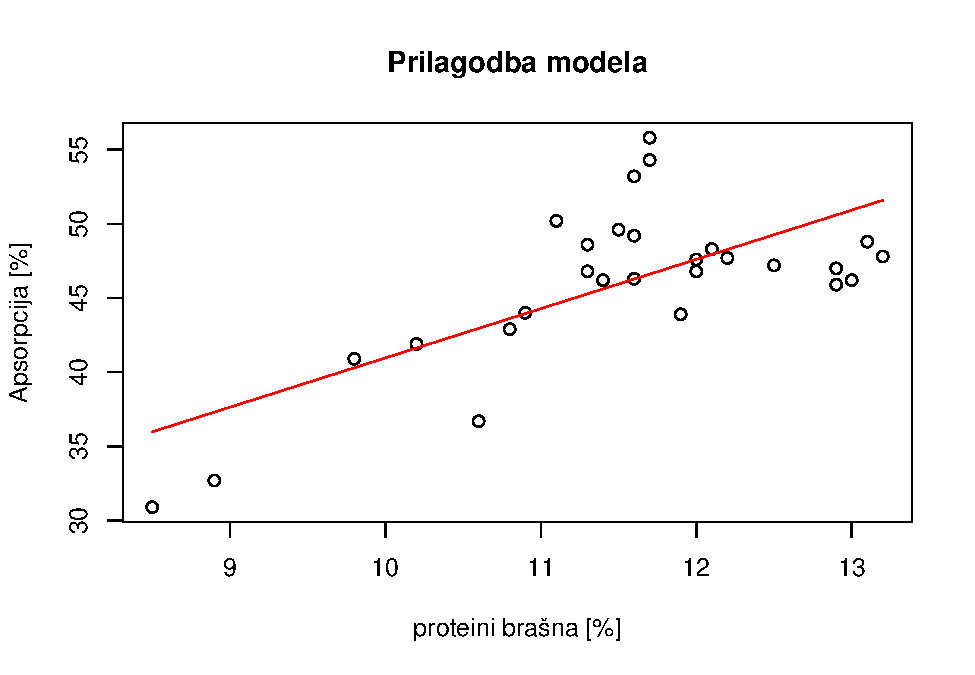
\includegraphics{Izvjestaj_files/figure-latex/unnamed-chunk-28-1.pdf}

\begin{Shaded}
\begin{Highlighting}[]
\KeywordTok{summary}\NormalTok{(model)}
\end{Highlighting}
\end{Shaded}

\begin{verbatim}
## 
## Call:
## lm(formula = Z ~ X)
## 
## Residuals:
##     Min      1Q  Median      3Q     Max 
## -6.2542 -3.4265  0.0108  1.8721  9.1928 
## 
## Coefficients:
##             Estimate Std. Error t value Pr(>|t|)    
## (Intercept)    7.753      7.877   0.984    0.334    
## X              3.321      0.681   4.876 4.66e-05 ***
## ---
## Signif. codes:  0 '***' 0.001 '**' 0.01 '*' 0.05 '.' 0.1 ' ' 1
## 
## Residual standard error: 4.113 on 26 degrees of freedom
## Multiple R-squared:  0.4777, Adjusted R-squared:  0.4576 
## F-statistic: 23.78 on 1 and 26 DF,  p-value: 4.656e-05
\end{verbatim}

Iz sažetka iznad doznajemo vrijednost statistike \(R^2\) koja iznosi
0.4777. Možemo biti zadovoljni dobivenim rezultatom.

Drugi model čiju ćemo prilagodbu provesti jest slijedeći linearni model:
\[z = \beta_0 + \beta_1 y \]

\begin{Shaded}
\begin{Highlighting}[]
\NormalTok{Y <-}\StringTok{ }\NormalTok{C.data$y}
\NormalTok{Z <-}\StringTok{ }\NormalTok{C.data$z}

\NormalTok{model2 <-}\StringTok{ }\KeywordTok{lm} \NormalTok{(Z ~}\StringTok{ }\NormalTok{Y)}
\end{Highlighting}
\end{Shaded}

Slijedeći graf prikazuje pravac dobiven prilagodbom navedenog modela
zajedno s empirijskim podacima. Dobili smo pravac
\(z = 0.39722*y + 34.21809\).

\begin{Shaded}
\begin{Highlighting}[]
\KeywordTok{plot}\NormalTok{(Y, Z, }\DataTypeTok{xlab =} \StringTok{"gubitak škroba [Farrandove jedinice]"}\NormalTok{, }\DataTypeTok{ylab =} \StringTok{"Apsorpcija [%]"}\NormalTok{,}
     \DataTypeTok{main=}\StringTok{"Prilagodba modela"}\NormalTok{)}
\KeywordTok{lines}\NormalTok{(Y, model2$fitted.values, }\DataTypeTok{col=}\StringTok{"red"}\NormalTok{)}
\end{Highlighting}
\end{Shaded}

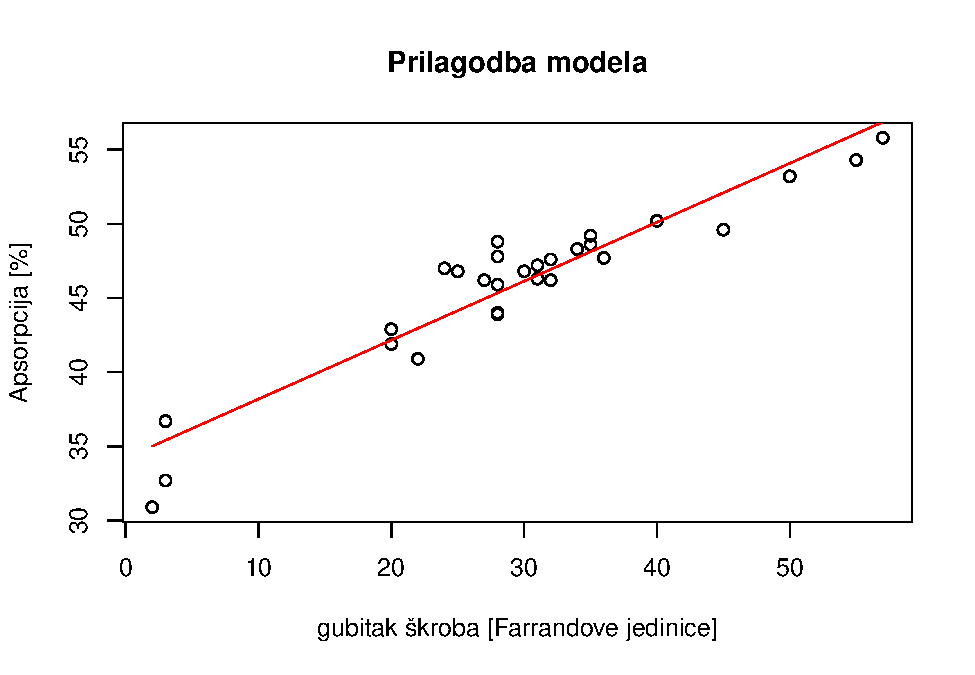
\includegraphics{Izvjestaj_files/figure-latex/unnamed-chunk-31-1.pdf}

\begin{Shaded}
\begin{Highlighting}[]
\KeywordTok{summary}\NormalTok{(model2)}
\end{Highlighting}
\end{Shaded}

\begin{verbatim}
## 
## Call:
## lm(formula = Z ~ Y)
## 
## Residuals:
##     Min      1Q  Median      3Q     Max 
## -4.1125 -1.1297  0.2862  0.8230  3.4598 
## 
## Coefficients:
##             Estimate Std. Error t value Pr(>|t|)    
## (Intercept) 34.21809    0.85941   39.82  < 2e-16 ***
## Y            0.39722    0.02655   14.96 2.75e-14 ***
## ---
## Signif. codes:  0 '***' 0.001 '**' 0.01 '*' 0.05 '.' 0.1 ' ' 1
## 
## Residual standard error: 1.836 on 26 degrees of freedom
## Multiple R-squared:  0.8959, Adjusted R-squared:  0.8919 
## F-statistic: 223.8 on 1 and 26 DF,  p-value: 2.751e-14
\end{verbatim}

Iz sažetka pripradnog modela možemo očitati vrijednost statistike
\(R^2\) koja iznosi 0.8959. Primjećujemo da je vrijednost statistike
\(R^2\) veća nego za prvi model čime možemo naslutiti da će koeficijent
uz varijablu x biti veći nego uz y u zadnjem modelu.

\subsection{Prilagodba linearnog modela s dvije nezavisne
varijable}\label{prilagodba-linearnog-modela-s-dvije-nezavisne-varijable}

Nakon što smo radili prilagodbe s jednom nezavisnom varijablom radimo
prilagodbu s dvije nezavisne varijable. Sljedeći model čiju ćemo
prilagodbu provesti jest sljedeći linearni model:
\[z = \theta_0 + \theta_1 x + \theta_2 y \]

\begin{Shaded}
\begin{Highlighting}[]
\NormalTok{X <-}\StringTok{ }\NormalTok{C.data$x}
\NormalTok{Y <-}\StringTok{ }\NormalTok{C.data$y}
\NormalTok{Z <-}\StringTok{ }\NormalTok{C.data$z}

\NormalTok{model3 <-}\StringTok{ }\KeywordTok{lm} \NormalTok{(Z ~}\StringTok{ }\NormalTok{Y +}\StringTok{ }\NormalTok{X)}
\end{Highlighting}
\end{Shaded}

\subsubsection{Značajnost dobivenog
modela}\label{znacajnost-dobivenog-modela}

\begin{Shaded}
\begin{Highlighting}[]
\KeywordTok{summary}\NormalTok{(model3)}
\end{Highlighting}
\end{Shaded}

\begin{verbatim}
## 
## Call:
## lm(formula = Z ~ Y + X)
## 
## Residuals:
##      Min       1Q   Median       3Q      Max 
## -2.10062 -0.60544 -0.03045  1.00419  1.66205 
## 
## Coefficients:
##             Estimate Std. Error t value Pr(>|t|)    
## (Intercept) 19.43976    2.18829   8.884 3.30e-09 ***
## Y            0.33563    0.01814  18.507 4.18e-16 ***
## X            1.44228    0.20764   6.946 2.79e-07 ***
## ---
## Signif. codes:  0 '***' 0.001 '**' 0.01 '*' 0.05 '.' 0.1 ' ' 1
## 
## Residual standard error: 1.094 on 25 degrees of freedom
## Multiple R-squared:  0.9645, Adjusted R-squared:  0.9616 
## F-statistic: 339.3 on 2 and 25 DF,  p-value: < 2.2e-16
\end{verbatim}

Iz sažetka očitavamo da je vrijednost statistike \(R^2\) = 0.9645. Pošto
su p-vrijednosti uz sve koeficijente jako male (X,Y) možemo zaključiti
da su oba koeficijenta iznimno značajna za naš model.

\subsubsection{Uspoređivanje proširenog modela s reduciranima koristeći
ANOVU}\label{usporeivanje-prosirenog-modela-s-reduciranima-koristeci-anovu}

\begin{Shaded}
\begin{Highlighting}[]
\KeywordTok{anova}\NormalTok{(model,model3)}
\end{Highlighting}
\end{Shaded}

\begin{verbatim}
## Analysis of Variance Table
## 
## Model 1: Z ~ X
## Model 2: Z ~ Y + X
##   Res.Df    RSS Df Sum of Sq     F    Pr(>F)    
## 1     26 439.93                                 
## 2     25  29.93  1    410.01 342.5 4.181e-16 ***
## ---
## Signif. codes:  0 '***' 0.001 '**' 0.01 '*' 0.05 '.' 0.1 ' ' 1
\end{verbatim}

\begin{Shaded}
\begin{Highlighting}[]
\KeywordTok{anova}\NormalTok{(model2,model3)}
\end{Highlighting}
\end{Shaded}

\begin{verbatim}
## Analysis of Variance Table
## 
## Model 1: Z ~ Y
## Model 2: Z ~ Y + X
##   Res.Df    RSS Df Sum of Sq     F    Pr(>F)    
## 1     26 87.687                                 
## 2     25 29.928  1     57.76 48.25 2.789e-07 ***
## ---
## Signif. codes:  0 '***' 0.001 '**' 0.01 '*' 0.05 '.' 0.1 ' ' 1
\end{verbatim}

Koristeći ANOVU usporedili smo prvi model \(z = \alpha_0 + \alpha_1 x \)
i treći model \(z = \theta_0 + \theta_1 x + \theta_2 y \). Pošto smo
dobili da je p-vrijednost jednaka \(4.181e-16\) možemo odbaciti hipotezu
da je novododani koeficijent jednak 0. Zaključujemo da je prošireni
model bolji od reduciranog. Zatim smo uspredili drugi model
\(z = \beta_0 + \beta_1 y \) i treći model
\(z = \theta_0 + \theta_1 x + \theta_2 y \). Ponovno smo dobili jaku
malu p-vrijednost koja iznosi \(2.789e-07\) te možemo odbaciti hipotezu
da podaci podržavaju reducirani oblik.

\subsection{Provjera normalnosti
reziduala}\label{provjera-normalnosti-reziduala-2}

Sljedeće što ćemo napraviti je provjeriti normalnost reziduala.
Koristimo ćemo sljedeća dva kriterija: grafički (QQ plot) te
Kolmogorov-Smirnovljev test.

Prvo ćemo nacrtati grafove reziduala i standardiziranih reziduala.

\begin{Shaded}
\begin{Highlighting}[]
\KeywordTok{plot}\NormalTok{(model3$residuals)}
\end{Highlighting}
\end{Shaded}

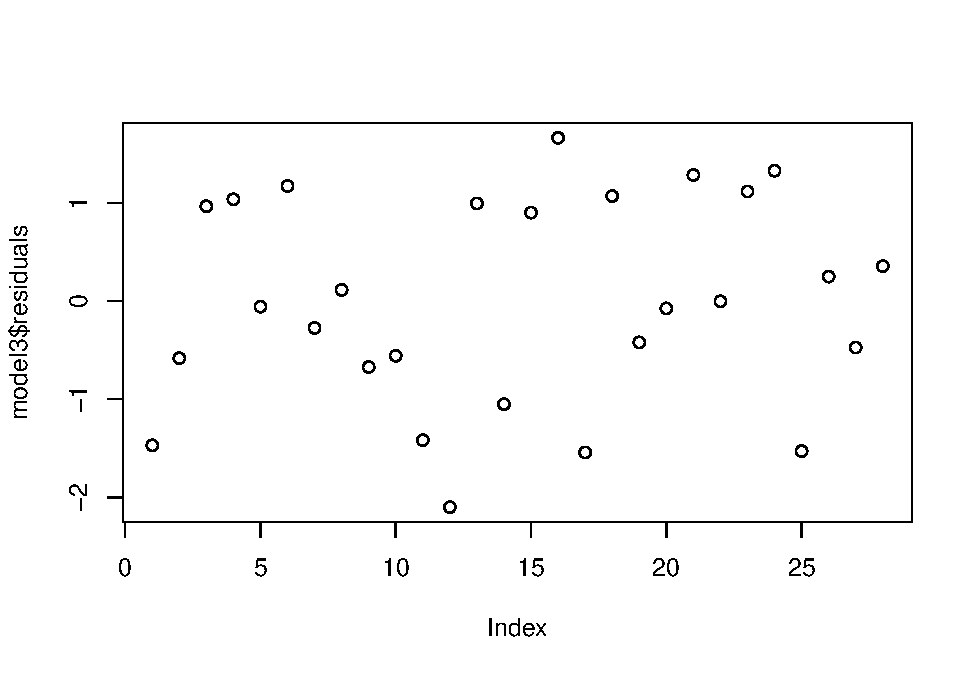
\includegraphics{Izvjestaj_files/figure-latex/unnamed-chunk-36-1.pdf}

\begin{Shaded}
\begin{Highlighting}[]
\KeywordTok{plot}\NormalTok{(}\KeywordTok{rstandard}\NormalTok{(model3))}
\end{Highlighting}
\end{Shaded}

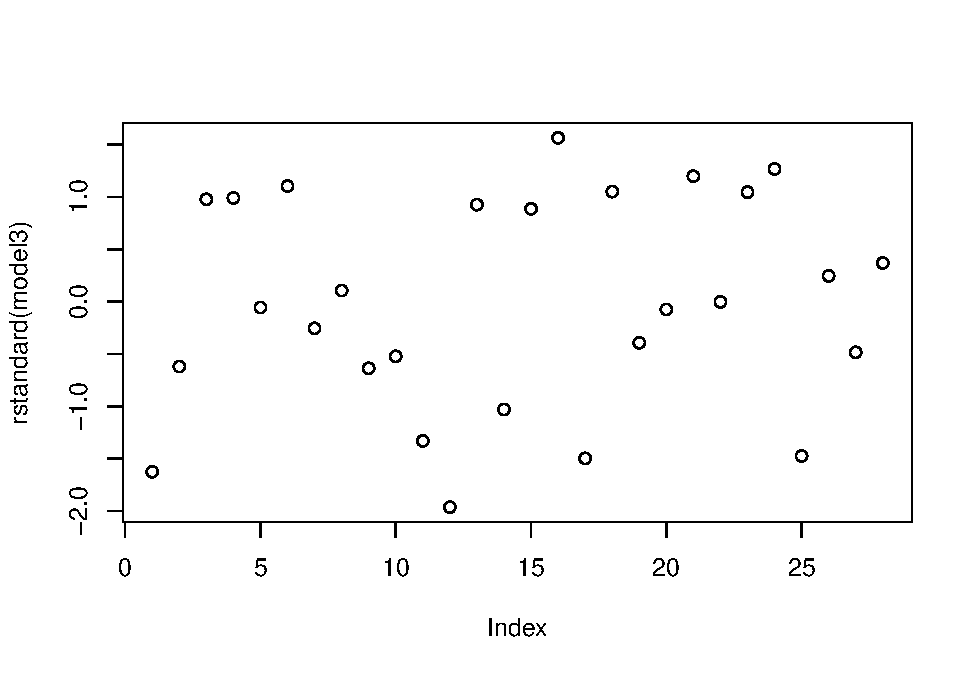
\includegraphics{Izvjestaj_files/figure-latex/unnamed-chunk-36-2.pdf}

\subsubsection{QQ plot}\label{qq-plot-3}

\begin{Shaded}
\begin{Highlighting}[]
\KeywordTok{qqnorm}\NormalTok{(}\KeywordTok{rstandard}\NormalTok{(model3), }\DataTypeTok{xlab =} \StringTok{'Teoretski kvantili'}\NormalTok{, }\DataTypeTok{ylab =} \StringTok{'Kvantili iz uzorka'}\NormalTok{,}
       \DataTypeTok{main =} \StringTok{'QQ plot'}\NormalTok{)}
\KeywordTok{abline}\NormalTok{(}\DataTypeTok{a=}\DecValTok{0}\NormalTok{,}\DataTypeTok{b=}\DecValTok{1}\NormalTok{)}
\end{Highlighting}
\end{Shaded}

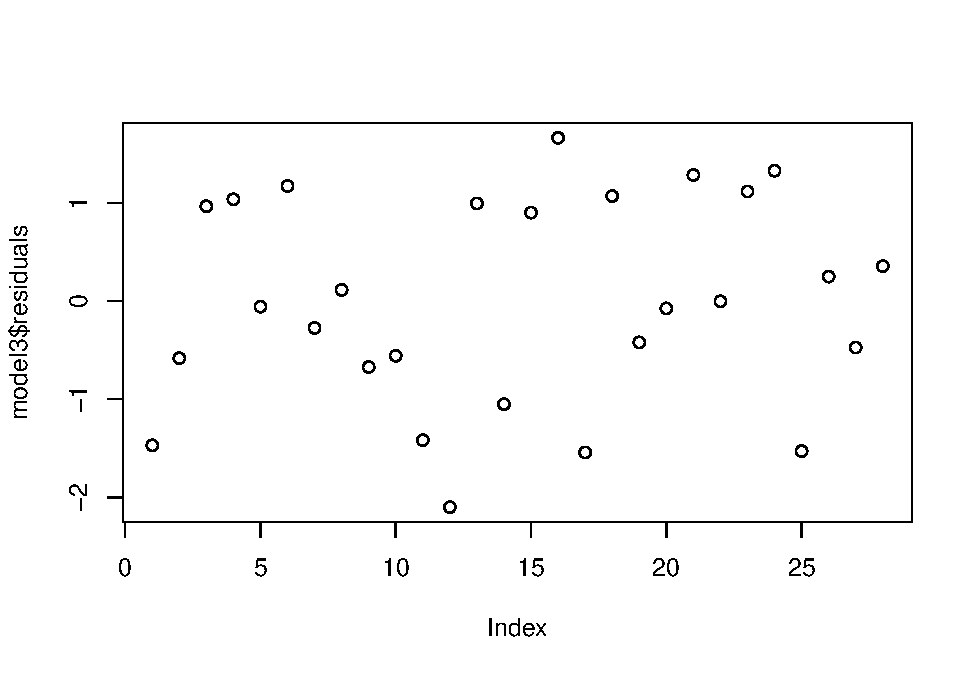
\includegraphics{Izvjestaj_files/figure-latex/unnamed-chunk-37-1.pdf}

Analizom dobivenog QQ plota možemo naslutiti da reziduale
najvjerojatnije dolaze iz normalne razdiobe. Kolmogorov-Smirnovljev test
bi to trebao potvrditi jer nam je veličina uzorka jako mala.

\subsubsection{Kolmogorov-Smirnovljev
test}\label{kolmogorov-smirnovljev-test-3}

\begin{Shaded}
\begin{Highlighting}[]
\KeywordTok{ks.test}\NormalTok{(}\KeywordTok{rstandard}\NormalTok{(model3), }\StringTok{'pnorm'}\NormalTok{)}
\end{Highlighting}
\end{Shaded}

\begin{verbatim}
## 
##  One-sample Kolmogorov-Smirnov test
## 
## data:  rstandard(model3)
## D = 0.16921, p-value = 0.3584
## alternative hypothesis: two-sided
\end{verbatim}

Rezultati Kolmogorov-Smirnov potvrđuju nam da podaci dolaze iz normalne
razdiobe pošto p-vrijednost iznosi 0.3584. Interpretacija dane
p-vrijednosti je da ne možemo odbaciti hipotezu da podaci dolaze iz
normalne razdiobe.

\subsection{Plohe 95\% pouzdanih
intervala}\label{plohe-95-pouzdanih-intervala}

Na sljedećem grafu su prikazani originalni podaci zajedno s plohama za
intervale predikcije (siva boja) i intervale pouzdanosti (crvena boja).

\begin{Shaded}
\begin{Highlighting}[]
\KeywordTok{require}\NormalTok{(scatterplot3d)}
\KeywordTok{require}\NormalTok{(plot3D)}
\end{Highlighting}
\end{Shaded}

\begin{verbatim}
## Loading required package: plot3D
\end{verbatim}

\begin{verbatim}
## Warning: package 'plot3D' was built under R version 3.3.3
\end{verbatim}

\begin{Shaded}
\begin{Highlighting}[]
\CommentTok{#scatterplot3d(X,Y,Z, pch = 19, color = "green4", main="3D Scatterplot")}
\NormalTok{X.new =}\StringTok{ }\KeywordTok{seq}\NormalTok{(}\KeywordTok{min}\NormalTok{(X), }\KeywordTok{max}\NormalTok{(X),}\DataTypeTok{length.out =} \DecValTok{1000}\NormalTok{)}
\NormalTok{Y.new =}\StringTok{ }\KeywordTok{seq}\NormalTok{(}\KeywordTok{min}\NormalTok{(Y), }\KeywordTok{max}\NormalTok{(Y),}\DataTypeTok{length.out =} \DecValTok{1000}\NormalTok{)}

\NormalTok{prediction <-}\StringTok{ }\KeywordTok{predict.lm}\NormalTok{(model3, }\DataTypeTok{newdata =} \KeywordTok{data.frame}\NormalTok{(}\DataTypeTok{X=}\NormalTok{X.new, }\DataTypeTok{Y=}\NormalTok{Y.new),}
                         \DataTypeTok{interval =} \StringTok{'prediction'}\NormalTok{, }\DataTypeTok{level=}\FloatTok{0.95}\NormalTok{)}
\NormalTok{confidence <-}\StringTok{ }\KeywordTok{predict.lm}\NormalTok{(model3, }\DataTypeTok{newdata =} \KeywordTok{data.frame}\NormalTok{(}\DataTypeTok{X=}\NormalTok{X.new, }\DataTypeTok{Y=}\NormalTok{Y.new),}
                         \DataTypeTok{interval =} \StringTok{'confidence'}\NormalTok{, }\DataTypeTok{level=}\FloatTok{0.95}\NormalTok{)}


\KeywordTok{scatter3D}\NormalTok{(X, Y, Z, }\DataTypeTok{colvar =} \OtherTok{NULL}\NormalTok{, }\DataTypeTok{col =} \StringTok{"blue"}\NormalTok{,}
          \DataTypeTok{pch =} \DecValTok{19}\NormalTok{, }\DataTypeTok{cex =} \FloatTok{0.5}\NormalTok{)}
\KeywordTok{scatter3D}\NormalTok{(X.new,Y.new,prediction[,}\DecValTok{2}\NormalTok{], }\DataTypeTok{add =} \OtherTok{TRUE}\NormalTok{, }\DataTypeTok{colkey =} \OtherTok{FALSE}\NormalTok{, }
         \DataTypeTok{pch =} \DecValTok{18}\NormalTok{, }\DataTypeTok{cex =} \DecValTok{3}\NormalTok{, }\DataTypeTok{col =} \StringTok{"gray"}\NormalTok{)}
\KeywordTok{scatter3D}\NormalTok{(X.new,Y.new,prediction[,}\DecValTok{3}\NormalTok{], }\DataTypeTok{add =} \OtherTok{TRUE}\NormalTok{, }\DataTypeTok{colkey =} \OtherTok{FALSE}\NormalTok{, }
         \DataTypeTok{pch =} \DecValTok{18}\NormalTok{, }\DataTypeTok{cex =} \DecValTok{3}\NormalTok{, }\DataTypeTok{col =} \StringTok{"gray"}\NormalTok{)}
\KeywordTok{scatter3D}\NormalTok{(X.new,Y.new,confidence[,}\DecValTok{2}\NormalTok{], }\DataTypeTok{add =} \OtherTok{TRUE}\NormalTok{, }\DataTypeTok{colkey =} \OtherTok{FALSE}\NormalTok{, }
         \DataTypeTok{pch =} \DecValTok{18}\NormalTok{, }\DataTypeTok{cex =} \DecValTok{3}\NormalTok{, }\DataTypeTok{col =} \StringTok{"red"}\NormalTok{)}
\KeywordTok{scatter3D}\NormalTok{(X.new,Y.new,confidence[,}\DecValTok{3}\NormalTok{], }\DataTypeTok{add =} \OtherTok{TRUE}\NormalTok{, }\DataTypeTok{colkey =} \OtherTok{FALSE}\NormalTok{, }
         \DataTypeTok{pch =} \DecValTok{18}\NormalTok{, }\DataTypeTok{cex =} \DecValTok{3}\NormalTok{, }\DataTypeTok{col =} \StringTok{"red"}\NormalTok{)}
\end{Highlighting}
\end{Shaded}

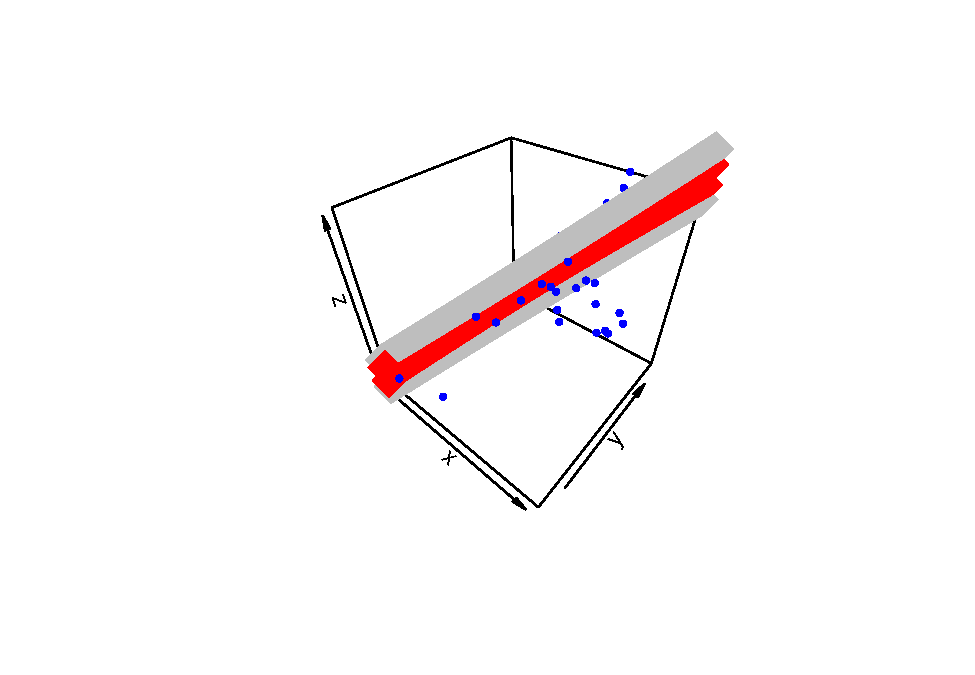
\includegraphics{Izvjestaj_files/figure-latex/unnamed-chunk-39-1.pdf}


\end{document}
